\documentclass[11pt]{article}
\usepackage{polski}
\usepackage[utf8]{inputenc}
\usepackage[a4paper, margin=20mm]{geometry}
\usepackage{amsmath}                        % Math symbols
\usepackage{amssymb}                        % More math symbols
\usepackage{graphicx}                       % Figures, images
\usepackage{subfigure}                      % Multiple figures in one
\usepackage{footnote}                       % Footnote on bottom of page
\usepackage{rotating}                       % Rotate figures by given angle
\usepackage{slantsc}                        % Small caps
\usepackage[hidelinks]{hyperref}            % Hyperlinks without red box
\usepackage{standalone}                     % import standalone docs
                                            % Mainly for tikz
\usepackage[T1]{fontenc}                    % Best text enocoding
\usepackage[newfloat]{minted}               % For code listings
\setminted{autogobble}                      % Remove unnecessary indents
\usepackage{siunitx}                        % SI Units
\DeclareSIUnit \amperehour { Ah }
\DeclareSIUnit \mil { mil }

\usepackage{tikz}                           % Graphing and plotting
\usetikzlibrary{shapes,                     % Tikz common shapes
				arrows}                     % Tikz common arrows
\tikzstyle{every node}=[font=\small]        % Make tikz globally prettier
\tikzstyle{every path}=[line width=0.8pt,
						line cap=round,
						line join=round]

\graphicspath{ {Graphics/} }
\author{Maciej Ziaja \and Bartosz Staszulonek}
\date{\today}

\begin{document}

\pagenumbering{gobble}
\title{
	Projekt Systemy Mikroprocesorowe \\
	\large MazeBot \\
	Robot unikający przeszkód z regulacją napędu silników prądu stałego}

\maketitle

\newpage
\pagenumbering{arabic}
\tableofcontents

\section{Wstęp}

\subsection{Abstrakt}
Projekt polega na konstrukcji mobilnego robota, który unika przeszkód.
Układ porusza się na dwóch kołach oraz wykrywa elementy otoczenia używając czujnika ultradźwiękowego zamocowanego na~wieży serwomechanizmu.
Platforma robota napędzana jest za pomocą pary silników prądu stałego, których kąt obrotu jest odczytywany przez czujniki szczelinowe.
W celu zwiększenia precyzji działania konstrukcji zbudowano układy regulacji prędkości silników.
Wykonano dwa typy układów regulacji: synchronizujący prędkość obrotu obu silników, w~celu zachowania kierunku jazdy na~wprost, oraz kaskadowy układ regulacji skrętu platformy robota.
Układ regulacji skrętu robota przypomina zasadą działania prosty serwomechanizm.
Przedstawiono metodę identyfikacji obiektu regulacji i~strojenia regulatorów z~użyciem linii pierwiastkowych.
Na potrzeby projektu wykonano także schemat układu elektronicznego i~zrealizowano go~w~postaci obwodu drukowanego \textsc{pcb}.
Zaprojektowano także podwozie robota i~wydrukowano je~w~technologii~3D.

\subsection{Cel i zakres projektu}
Projekt obejmował budowę platformy bazującej na~mikroprocesorze z~serii ATmega32, obsługującym peryferia:
\begin{itemize}
	\item czujnika ultradźwiękowego wykrywającego przeszkody,
	\item wieży serwomechanizmu, na której zamontowany jest czujnik i~która kieruje go w~różne strony,
	\item silników prądu stałego stanowiących napęd platformy,
	\item czujników szczelinowych odczytujących kąt obrotu kół platformy,
	\item odbiornika podczerwieni pozwalającego na~zdalne wyłączenie robota, jeśli ten się oddali.
\end{itemize}
Współpraca wymienionych komponentów pozwala robotowi na unikanie przeszkód.
Działanie robota powinno polegać na~jeździe przed siebie, do~czasu napotkania przeszkody.
W~momencie wykrycia przeszkody robot powinien się zatrzymać, a~następnie zbadać czy w~jego otoczeniu znajduje się niezagrodzona droga i~skierować się w jej stronę.
Prototyp układu wykonano z~użyciem układu Arduino Leonardo.
Na wykonanym prototypie wykonano testy współpracy komponentów i~wyciągnięto wnioski dotyczące budowy finalnej konstrukcji oraz wymaganych parametrów komponentów.
Działanie prototypu prowadziło do następujących decyzji projektowych, które podyktowały dalszy tok projektu i~jego zakres:
\begin{itemize}
	\item w~celu wydajnego wykorzystania przestrzeni na platformie zdecydowano się na wykonanie własnego układu elektronicznego i~obwodu drukowanego,
	\item zaprojektowano własne podwozie dopasowane do~używanych peryferiów,
	\item wykonano układy regulacji jazdy na wprost oraz skręcania platformy.
\end{itemize}

\section{Organizacja projektu}
\subsection{Harmonogram}
Projekt należało zrealizować w przeciągu 4 miesięcy.
Proces jego wykonania składał się z~dwóch części: testów komponentów wraz z~budową prototypu oraz konstrukcji finalnego układu, na~podstawie wniosków wyciągniętych z~testów konstrukcji prototypowej.
	Tabela \ref{tab:sched} przedstawia ramowy rozkład pracy w~czasie.

\begin{table}[hbt]
	\centering
	\begin{tabular}{|c|c|}
	\hline
Termin                  & Zakres pracy                                                                         \\ \hline
01.10.2018 - 20.10.2018 & Zebranie komponentów układu, ustalenie zakresu prac                                  \\ \hline
20.10.2018 - 01.11.2018 & Test komponentów i~peryferiów z użyciem Arduino Leonardo                             \\ \hline
01.11.2018 - 14.11.2018 & Budowa prototypu, programowanie głównej logiki programu \\ \hline
14.11.2018 - 01.12.2018 & Projekty obwodu drukowanego PCB i~podwozia                                           \\ \hline
01.12.2018 - 20.12.2018 & Synteza i~oprogramowanie układów regulacji                                           \\ \hline
20.12.2018 - 01.01.2019 & Złożenie finalnego układu                                                            \\ \hline
01.01.2019 - 20.01.2019 & Strojenie układów regulacji, budowa dokumentacji                                      \\ \hline
	\end{tabular}
	\caption{Harmonogram pracy}
	\label{tab:sched}
\end{table}

\subsection{Budżet}
Budżet projektu wynosił 150 złotych, najbardziej znaczącym wydatkiem w~projekcie było wydrukowanie obwodu elektronicznego.
Zaletą projektu jest modułowość konstrukcji podwozia, przez co~elementy można łatwo wymieniać w~przypadku chęci zastosowania droższych lub tańszych komponentów.
Finalny kosztorys projektu przedstawia tabela \ref{tab:budget}, dokładny spis elementów elektronicznych na~obwodzie drukowanym przedstawiono w~dokumencie \textsc{csv} załączonym do plików projektu.
Całkowity koszt komponentów projektu wyniósł 149,86 złotych.

\begin{table}[hbt]
	\centering
	\begin{tabular}{|c|c|c|c|}
		\hline
		Komponent                                                                                    & Koszt     & Producent                                                           & Dostawca                  \\ \hline
		Obwód drukowany PCB                                                                          & 53,00 PLN    & Elpin PCB                                                           & Elpin PCB                 \\ \hline
		ATmega32u4                                                                                   & 15,91 PLN & Microchip Atmel                                                     & TME Electronic Components \\ \hline
		Elementy pasywne                                                                             & $\backsim$7,50 PLN    & \begin{tabular}[c]{@{}c@{}}Panasonic,\\ ST Electronics\end{tabular} & TME Electronic Components \\ \hline
		Elementy aktywne                                                                             & $\backsim$4,00 PLN     & ST Electronics                                                      & TME Electronic Components \\ \hline
		\begin{tabular}[c]{@{}c@{}}Silniki prądu stałego\\ z kołami i dyskami enkoderów\end{tabular} & 19,90 PLN & Dagu                                                                & Botland                   \\ \hline
		Serwomechanizm                                                                               & 6,90 PLN  & Tower Pro                                                           & Botland                   \\ \hline
		\begin{tabular}[c]{@{}c@{}}Ultradźwiękowy czujnik\\ odległości HC-SR04\end{tabular}          & 7,90 PLN  & Elec                                                                & Botland                   \\ \hline
		Czujniki szczelinowe                                                                         & 9,90 PLN  & Vishay                                                              & Botland                   \\ \hline
		\begin{tabular}[c]{@{}c@{}}Odbiornik podczerwieni\\ TSOP4836 - 36khz\end{tabular}            & 2,95 PLN  & Vishay                                                              & Botland                   \\ \hline
		Bateria Li-Pol                                                                               & 21,90 PLN & Dualsky                                                             & Botland                   \\ \hline
\end{tabular}
	\caption{Kosztorys, rozdysponowanie budżetu}
	\label{tab:budget}
\end{table}


\section{Budowa prototypu, analiza problemów}
Realizację projektu zaczęto od~zgromadzenia peryferiów koniecznych do~realizacji konstrukcji robota.
W~pierwszej fazie prototypowania komponenty testowano osobno używając Arduino Leonardo. Zapoznano się z~ich praktycznymi możliwościami i~działaniem dostępnych bibliotek. 

Następnie połączono wszystkie komponenty i~przeprowadzono ich jednoczesne testy oraz zmierzono zasilanie używając multimetru wraz z~zasilaczem regulowanym.
Elementy prototypowe umieszczono na~platformie testowej i oceniono działanie konstrukcji.
Okazało się, że działanie robota jest możliwe, ale sterowanie silnikami w~torze otwartym nie było wystarczająco precyzyjne aby unikać przeszkód. Przy symetrycznym wysterowaniu silników robot nie poruszał się w~kierunku prostym, różnice w działaniu poszczególnych silników są~zbyt duże by~pracowały one symetrycznie co jest wymagane by platforma jechała na~wprost.
Skręcanie platformy o~zadany kąt również okazało się nieprecyzyjne, obroty o~na~przykład 90~stopni w~prawo były mało powtarzalne i~obarczone dużym błędem.
Zdecydowano się na~syntezę układów regulacji, aby wyeliminować te~problemy.

Testy platformy prototypowej pokazały także, że~złożoność układu jest zbyt duża aby budować go~na~płytce stykowej/prototypowej.
Dodatkowo serwomechanizm, który jest bardzo wrażliwy na~zakłócenia zasilania, działał źle gdy był połączony przez wiele kabli, które razem tworzyły dużą rezystancję. Obserwacje te~skłoniły nas do~zaprojektowania własnego obwodu drukowanego, który mieściłby wszystkie potrzebne komponenty elektroniczne na małej przestrzeni.
Konstrukcja mechaniczna platformy prototypowej okazała się mało solidna i~nie była dostosowana do~używanych przez nas modułów elektronicznych. W~celu zwiększenia  wytrzymałości i~schludności wykonania układu zdecydowano się na~projekt własnego podwozia robota.

\section{Projekt układu elektronicznego}
\subsection{Działanie i uzasadnienie doboru elementów elektronicznych}
\subsubsection{Mikroprocesor ATmega32u4}
Centralnym elementem robota jest mikroprocesor \textsc{avr} o~architekturze \textsc{risc}. Ośmiobitowe mikroprocesory ATmega są~popularnym wyborem przy konstrukcji układów wbudowanych w~przemyśle i~urządzeniach elektronicznych o~niedużym stopniu wymaganej wydajności.
Ich~zaletą jest powszechność oraz fakt,~że~na~procesorach z~tej rodziny bazuje popularna platforma Arduino, w~ramach której dostępny jest szeroki zakres bibliotek programistycznych do~obsługi peryferiów. 

\noindent\begin{minipage}{\linewidth}
Przy wyborze konkretnego modelu mikroprocesora kierowaliśmy się następującymi wymaganiami:
\begin{itemize}
	\item obsługa czterech przerwań zewnętrznych:
		\begin{enumerate}
			\item pochodzących z~enkodera lewego koła,
			\item pochodzących z~enkodera prawego koła,
			\item pochodzących z~czujnika ultradźwiękowego,
			\item pochodzących z~odbiornika podczerwieni, 
		\end{enumerate}
	\item obsługa trzech wyjść PWM, za~pomocą liczników w~celu:
		\begin{enumerate}
			\item sterowania prędkością lewego silnika prądu stałego,
			\item sterowania prędkością prawego silnika prądu stałego,
			\item sterowania położeniem serwomechanizmu, na~którym zamontowany jest czujnik ultradźwiękowy,
		\end{enumerate}
	\item możliwość użycia sumarycznie dwunastu wejść wyjść cyfrowych do~komunikacji z~peryferiami,
	\item pożądana jest wbudowana obsługa komunikacji szeregowej za~pomocą interfejsu USB w~celu łatwego debugowania układu i~zdjęcia pomiarów dynamiki układu przy identyfikacji obiektu regulacji i~strojeniu regulatorów,
	\item powyższe wymagania powinny być spełnione przy użyciu bootloadera i~bibliotek Arduino.
\end{itemize}
\hspace{5mm}
\end{minipage}

Powyższe wymagania spełnia mikroprocesor ATmega32u4 firmy Atmel, co~można wywnioskować z~jego dokumentacji \cite{atmega32u4_datasheet}.
Na~tym procesorze bazuje układ Arduino Leonardo, który wykorzystano przy konstrukcji prototypu.
Mikroprocesor ATmega32u4 z~użyciem bibliotek Arduino pozwala na~używanie do~pięciu przerwań zewnętrznych oraz siedmiu kanałów generujących sygnały \textsc{pwm}.

Istotne jest, że~kanały \textsc{pwm} są~obsługiwane przez cztery oddzielne liczniki. Biblioteki Arduino (szczególnie obsługi serwomechanizmu) wchodzą łatwo w~konflikty i~korzystają z~liczników w~sposób uniemożliwiający ich współdzielenie przy generowaniu sygnałów \textsc{pwm}.
Dlatego przy doborze mikroprocesora i~rozdysponowaniu jego zasobów starano się, aby serwomechanizm był obsługiwany przez oddzielny licznik, który nie jest dzielony z~innymi funkcjami układu.
Oznacza to,~że~pin sterujący serwem~nie powinien generować sygnałów z~użyciem tego samego licznika,~co inne kanały PWM, aby uniknąć konfliktów bibliotek Arduino.

Wybrany model mikroprocesora jest dostępny tylko w~obudowach powierzchniowych \textsc{qfp} (\textit{Quad Flat Package}), przy wyborze tej jednostki należy pamiętać, że wymaga ona umiejętności precyzyjnego lutowania. Procesor może pracować przy zasilaniu 5~\si{\volt}, jest to~dogodna wartość ponieważ reszta peryferiów w~układzie ma~takie same napięcie zasilania.

\subsubsection{Silniki prądu stałego}
Ze względu na ograniczenia budżetowe zdecydowano się na~jedne z najtańszych dostępnych silników, wyprodukowane przez firmę Dagu.
Silniki prądu stałego oferują największe momenty siły przy małych obrotach, nadają się dobrze do~napędzania i~przyspieszania platform robotów, oferują możliwość płynnego sterowania.
Ich wadą jest fakt, że bez dodatkowego układu czujników nie można określić ich kąta obrotu.
Należy mieć na uwadze, że~ze~względu na~obecność komutatora i~szczotek silniki prądu stałego zużywają się w~czasie pracy.
Parametry wybranych przez nas silników są~następujące:
\begin{itemize}
	\item maksymalne napięcie zasilania: 6~\si{\volt},
	\item moment obrotowy: \SI[inter-unit-product =\ensuremath{\cdot}]{0,8}{\kilogram\centi\meter}, \SI[inter-unit-product =\ensuremath{\cdot}]{0,78}{\newton\meter},
	\item obroty silnika bez obciążenia: $ (90 \pm 10) \ \frac{obr}{min} $,
	\item pobór prądu silnika bez obciążenia: 190~\si{\milli\ampere} (max. 250~\si{\milli\ampere}),
	\item pobór prądu silnika przy zatrzymanym wale: 1~\si{\ampere}.
\end{itemize}
Do silników przymocowano koła o parametrach:
\begin{itemize}
	\item średnicy: 65~\si{\milli\meter},
	\item szerokości: 30~\si{\milli\meter}.
\end{itemize}

\subsubsection{Sterownik silników prądu stałego -  mostek \textsc{h}}
Najbardziej popularnym sposobem sterowania silnikami prądu stałego jest użycie mostka~\textsc{h}.
~Jest to~układ składający się z~czterech tranzystorów polowych, których dreny i~źrodła są~odpowiednio połączone ze~sterowanym silnikiem. Para tranzystorów połączona z~tą samą szczotką silnika ma~złączone bramki, ale przeciwny stan otwarcia.
Złączone bramki są wyprowadzone z~układu i~stanowią wejścia sterowania. W~zależności od tego na które z~wejść podamy stan wysoki przez jeden z~tranzystorów z~każdej pary będzie płynął prąd, powodując obroty silnika w~odpowiednim kierunku.
Układem elektronicznym, który zawiera w sobie dwa mostki~\textsc{h},~co~pozwala na~sterowanie parą silników, jest L298N.
Dodatkowo układ posiada dodatkowe tranzystory do sterowania prędkością silników za pomocą sygnału \textsc{pwm}, który stopniowo otwiera i~domyka tranzystor polowy przepuszczający sygnały wejściowe. Parametry sterownika są~następujące:
\begin{itemize}
	\item maksymalne napięcie zasilania silników: 45~\si{\volt},
	\item napięcie części logicznej: od 4,5~\si{\volt} do 7~\si{\volt},
	\item maksymalny prąd zasilający silnik: 2~\si{\ampere}.
\end{itemize}
Sterownik dostępny jest w~obudowie przewlekanej \textit{Multiwatt15}, jego producentem jest firma STMicroelectronics. Porównując parametry mostka, zawarte w dokumentacji \cite{h_bridge_datasheet} z~parametrami silników możemy stwierdzić, że~jest on~wystarczający do~ich wysterowania.

\subsubsection{Czujnik ultradźwiękowy}
Najbardziej popularnym i~łatwo dostępnym miernikiem odległości jest czujnik ultradźwiękowy HC-SR04.
Czujniki ultradźwiękowe mierzą odległość na~podstawie czasu, który jest potrzebny fali ultradźwiękowej na~dotarcie do~przeszkody i~powrót do~czujnika po~jej odbiciu.
Pomiar czujnikiem rozpoczyna się od~podania na~wejście \textsc{trig} stanu wysokiego przez~10~\si{\micro\second}. Powoduje to~wygenerowanie przez czujnik ciągu ośmiu sygnałów ultradźwiękowych o~częstotliwości 40~\si{\kilo\hertz}. Po~odbiciu sygnału od przeszkody i~jego powrocie do~czujnika odległość można obliczyć według wzoru \ref{eq:ultrasonic}, gdzie:
\begin{itemize}
	\item $ d $ to odległość mierzona,
	\item $ t_h $ to czas trwania stanu wysokiego, 
	\item $ v_s $ to prędkość rozchodzenia się fali dźwiękowej w~powietrzu, typowo 340~\si{\meter\per\second}.
\end{itemize}
\begin{equation}
\label{eq:ultrasonic}
	d = \frac{t_h \cdot v_s}{2}
\end{equation}
Model czujnika HC-SR04, zgodnie z~dokumentacją \cite{ultr_datasheet} charakteryzuje się następującymi parametrami:
\begin{itemize}
	\item napięcie zasilania: 5~\si{\volt},
	\item średni pobór prądu: 15~\si{\milli\ampere},
	\item zakres pomiarowy: od 2~\si{\centi\meter} do 200~\si{\centi\meter},
	\item częstotliwość pracy: 40~\si{\kilo\hertz},
	\item wymiary: $ 45 \times 20 \times 15 $~\si{\milli\meter}.
\end{itemize}
Zasilanie czujnika  i~jego zakres pracy są odpowiednie dla projektu.
Przeszkody, które chcemy wykrywać będą znajdywały się w~odległości parunastu centymetrów od~robota, czyli w~zakresie pracy czujnika.
Należy mieć na uwadze, że~czujniki ultradźwiękowe wykrywają najlepiej duże przeszkody. 
Dodatkowo istotne jest, że~pomiar czujnika ultradźwiękowego trwa w~czasie, przebycie odpowiedniej drogi przez falę ultradźwiękową nie~jest natychmiastowe.
Kwestia ta~zostanie wzięta pod uwagę w~czasie tworzenia oprogramowania.

\subsubsection{Serwomechanizm}
Aby umożliwić robotowi kierowanie czujnika odległości w~różnych kierunkach, został on~zamieszczono na~wieży serwomechanizmu.
Ponieważ wymagamy aby czujnik mógł być skierowany w~lewo, prawo oraz na~wprost wystarczające jest serwo 180 stopni.
Waga czujnika ultradźwiękowego jest znikoma, dlatego serwomechanizm można wybrać kierując się jak najniższą ceną.

\subsubsection{Odbiornik podczerwieni TSOP4836}
Robota wyposażono w~odbiornik podczerwieni ułatwiający jego zatrzymanie.
W celu łatwej współpracy z~domowymi pilotami na~podczerwień należało wybrać odbiornik wspierający popularne formaty: NEC Code, Toshiba Micom Format, Sharp Code, RC5 Code, RC6 Code, R–2000 Code\dots.

Wybraliśmy odbiornik TSOP4836 pracujący z~falami o~częstotliwości 36~\si{\kilo\hertz}. Zgodnie z dokumentacją \cite{ir_datasheet} firmy Vishay
 odbiornika należy go~zabezpieczyć kondensatorem filtrującym i~rezystorem. Parametry odbiornika są~następujące:
\begin{itemize}
	\item napięcie zasilania: od 4,5~\si{\volt} do 5,5~\si{\volt},
	\item średni pobór prądu: 1,5~\si{\milli\ampere}.
\end{itemize}
Przy projektowaniu obwodu drukowanego i~lutowaniu odbiernika należy zwrócić uwagę na jego wyprowadzenia.
Wiele czujników podczerwieni o~identycznych obudowach i~podobnych parametrach ma~bardzo różne kolejności wyprowadzeń.

\subsubsection{Stabilizator napięcia L7805CV}
W konstruowanym projekcie wszystkie układy logiczne zasilane są~napięciem 5~\si{\volt}, natomiast silniki zasilane są napięciem  7,4~\si{\volt}.
Wynika stąd, że~najlepiej zastosować baterię siedmiowoltową, a~zasilanie części logicznej dostarczać poprzez regulator napięcia. Najbardziej popularnym regulatorem jest układ 7805,~produkowany przez firmę STMicroelectronics \cite{stab_datasheet}. 
W wersji \textsc{cv} jego parametry są następujące:
\begin{itemize}
	\item maksymalne napięcie wejściowe: 35~\si{\volt}$ 35\ V $,
	\item napięcie wyjściowe: 5~\si{\volt} (z dokładnością 2 \%),
	\item maksymalny prąd wyjściowy: 1,5~\si{\ampere}.
\end{itemize}
Stabilizator jest dostępny w~różnych obudowach, przewlekanych i~powierzchniowych. Ze~względu na~łatwość montażu, dostępność i~możliwość zamontowania radiatora wybraliśmy model w~obudowie przewlekanej~TO-220.
Po~porównaniu parametrów stabilizatora z~parametrami komponentów, które zasili można stwierdzić, że~jest on~wystarczający by~spełnić zapotrzebowania projektu.

\subsubsection{Akumulator}
Testy pokazały, że~przy zasilaniu 7,4~\si{\volt} układ pobiera prąd~do~0,3~\si{\ampere},~co dostarcza nam informacji potrzebnych do~doboru baterii dla robota.
Zdecydowano się na~zastosowanie akumulatora litowo-polimerowego firmy Dualsky.
Jego najważniejsze parametry są~następujące:
\begin{itemize}
	\item akumulator składa się z dwóch ogniw Li-pol,
	\item napięcie nominalne: 7,4~\si{\volt},
	\item pojemność: 800~\si{\milli\amperehour},
	\item prąd rozładowania ciągły: 20~\si{\ampere},
	\item wbudowane przewody ze wtykiem \textsc{jst}.
\end{itemize}

\subsubsection{Elementy pasywne}
Użyte komponenty elektroniczne wymagają użycia kondensatorów filtrujących, zastosowano kondensatory o~pojemnościach podanych w~dokumentacjach filtrowanych elementów.
Kondensatory ceramiczne są~umieszczone w~obudowach przewlekanych, starano się dobrać kondensatory elektrolityczne w~obudowach powierzchniowych, aby zredukować miejsce, którą zajmują.
Spis wszystkich elementów układu, w~tym elementów pasywnych znajduje się~w osobnym pliku \texttt{csv} dostępnym na stronie projektu.
\subsection{Schemat układu elektronicznego}
\label{sec:schem}

\begin{sidewaysfigure}[!htbp]
		\centering
		\includegraphics[scale=0.9]{"MazeBot Main Board".pdf}
		\caption{Schemat układu elektronicznego}
		\label{fig:sch_eletr}
\end{sidewaysfigure}

Na rysunku \ref{fig:sch_eletr} przedstawiono utworzony schemat układu elektronicznego.
Projekt układu wykonano w~programie Autodesk Eagle\footnote{Autodesk Eagle: \url{https://www.autodesk.com/products/fusion-360/overview}}, korzystając z~bibliotek komponentów. 

Centralnym elementem układu jest mikroprocesor ATmega32u4 oznaczony symbolem \textit{U3}, znajduje się on~w~polu \textit{C3} schematu.
Źródłem taktowania mikroprocesora jest zewnętrzny rezonator kwarcowy 16~\si{\mega\hertz}.
Do~jego poprawnego działania konieczne są~odpowiednie kondensatory.
Aby osiągnąć zamierzone taktowanie użyto kondensatorów o~pojemności 22~\si{\pico\farad}.
Mikroprocesor zasilono napięciem 5~\si{\volt},~które jest filtrowane kondensatorami 0,1~\si{\micro\farad},~zasilanie portu USB jest filtrowane kondensatorami 1~\si{\micro\farad}.
Aby ułatwić restartowanie układu, na schemacie umieszczono przycisk, który umożliwia zwieranie pinu reset z~ziemią.
Jeżeli przycisk jest przytrzymany dostatecznie długo układ mikroprocesorowy zostanie zresetowany.
Aby podczas resetu nie doszło do~zwarcia obwodu zasilania, dodano rezystor \textit{R1}.
Układ resetu znajduje się w~polu \textit{B2} schematu.

W polu \textit{A2} schematu umieszczono diody sygnalizacyjne.
Dioda \textit{PWR\_LED} sygnalizuje obecność napięcia na~wyjściu stabilizatora.
Diody \textit{TX\_LED} oraz \textit{RX\_LED} są związane~z~transmisją szeregową, podłączono je~tak że~są~aktywne kiedy wyjścia procesora są~w~stanie niskim.
Dzięki temu diody świecą kiedy transmisja szeregowa nie ma~miejsca i~sygnalizują tym samym poprawne działanie procesora.
Jest to~wygodne ponieważ dioda \textit{PWR\_LED} sygnalizuje jedynie obecność zasilania układu, ale nie informuje użytkownika o~właściwym uruchomieniu mikroprocesora.
Każda z~diod podłączona jest przez odpowiedni rezystor ograniczający płynący prąd.
W~polu \textit{C1} znajduje się port USB w wersji \textsc{micro}. Linie portu szeregowego zabezpieczono dławikiem ferrytowym, oraz rezystorami.
Do programowania mikroprocesora zastosowano złącze ICSP sześciopinowe, znajdujące się w~polu \textit{D1} schematu.

W~polu \textit{A5} schematu znajduje się mostek L298.
Aby zabezpieczyć układ do~jego wyjść silnikowych dodano diody prostownicze skierowane przeciwnie do~polaryzacji baterii.
W czasie pracy silników na~ich uzwojeniu gromadzi się energia w~postaci pola magnetycznego.
Po zatrzymaniu silników i~hamowaniu platformy energia to wróci do układu w~postaci płynącego prądu.
Dzięki obecności diod układ mostka jest zabezpieczony przez tymi prądami, popłyną one przez diody do~baterii.
 Co więcej, ze~względu na polaryzację diod, energia odzyskiwana z~silników będzie ładować baterię, tworząc prosty układ aktywnego hamowania.
W sekcji \textsc{io ports} znajdują się złącza peryferiów układu.


Komponenty z~fabrycznymi wyprowadzeniami przez goldpiny, połączono takimi samymi złączami od~strony układu.
Silniki i~zasilanie są złączone przez konektory \textsc{arc} dokręcane śrubokrętem.

\subsection{Projekt układu drukowanego}
\subsubsection{Parametry techniczne układu drukowanego}
Ze względu na~ograniczoną przestrzeń na~powierzchni platformy robota zdecydowano się na~wykonanie własnego obwodu drukowanego w~technologii dwustronnej, z~metalizowanymi otworami i~soldermaską.
W celu zachowania zgodności z procesem technologicznym producenta płytek\footnote{Elpin: \url{https://www.elpinpcb.com.pl/prototypy/}}
przyjęto następujące ustawienia \textsc{drc} (\textit{Design rules check}):
\begin{itemize}
	\item grubość laminatu wraz ze~ścieżkami: 1,5~\si{\milli\meter},
	\item grubość ścieżek: 0.035~\si{\milli\meter},
	\item odległości między ścieżkami, przelotkami (\textit{via}) oraz padami: 6~\si{\mil},
	\item odległości ścieżek od~krawędzi płytki: 40\si{\mil},
	\item minimalna odległość otworów: 6~\si{\mil},
	\item minimalna szerokość ścieżki: 6~\si{\mil},,
	\item minimalna średnica otworu: 0,35\si{\milli\meter},
	\item szerokość termoizolacji padów od~wylewek (ułatwia lutowanie): 10\si{\mil}.
\end{itemize}
Dwuwymiarowe wizualizacje obwodu drukowanego wykonanego w~programie Autodesk Eagle przedstawiają rysunki \ref{fig:pcb_top} oraz \ref{fig:pcb_bottom}.
Przy tworzeniu płytki zastosowano technikę wylewki masy, czyli tworzenia dużych płaszczyzn przewodnika, zamiast prowadzenia poszczególnych ścieżek.
Ułatwia to~rozmieszczenie połączeń i~zmniejsza rezystancję ścieżek masy.
Zastosowano materiały zawierające ołów jako bardziej wytrzymałe i~łatwiejsze w~lutowaniu.
W~amatorskim lutowaniu nie używa się temperatur przy których wydzielają się trujące opary ołowiu.

\begin{figure}[!htbp]
	\centering
	\includegraphics[width=\linewidth]{"MazeBot Main Board Top".png}
	\caption{Górna warstwa obwodu drukowanego}
	\label{fig:pcb_top}
\end{figure}

\begin{figure}[!htbp]
	\centering
	\includegraphics[width=\linewidth]{"MazeBot Main Board Bottom".png}
	\caption{Dolna warstwa obwodu drukowanego}
	\label{fig:pcb_bottom}
\end{figure}

\subsubsection{Rozmieszczenie elementów na powierzchni układu drukowanego}
W centralnej części obwodu drukowanego umieszczono mikroprocesor.
Rozdysponowanie wyprowadzeń sygnałowych mikroprocesora jest kompromisem między ograniczeniami bibliotek Arduino, możliwościami procesora oraz ilością miejsca dostępnego na~płytce.
Górną krawędź układu zajmują konektory peryferiów, dolna krawędź została przeznaczona na elementy służące interakcji z~użytkownikiem.
Płytka została wykonana w~technologii mieszanej\footnote{To znaczy użyto zarówno elementów przewlekanych jak i montowanych powierzchniowo}, w~celu zaoszczędzenia miejsca starano się używać elementów montowanych powierzchniowo, tam gdzie było to~możliwe i~wygodne.
Podczas prowadzenia ścieżek układu należy mieć na~uwadze ich szerokość.
Znając parametry techniczne płytki oraz prądy płynące przez poszczególne ścieżki można obliczyć ich minimalną szerokość za pomocą kalkulatorów dostępnych online\footnote{Kalkulator scieżek \textit{4PCB} \url{https://www.4pcb.com/trace-width-calculator.html}}.
Obudowę rezonatora kwarcowego oddzielono od~powierzchni obwodu wyciętą gumą.
Na~obudowach elementów aktywnych umieszczono radiatory.

\section{Projekt podwozia robota}
W~celu zwiększenia trwałości i~solidności budowy podwozia zdecydowano się zaprojektować własne oraz wydrukować je~w~technologii 3D.
Do jego modelowania użyto programu Autodesk Fusion 360\footnote{Autodesk Fusion 360: \url{https://www.autodesk.com/products/fusion-360/overview}}.
Podwozie zaprojektowano tak aby osiągnąć jego modułowość.
Platforma robota składa się z~osobnych części:
\begin{itemize}
	\item głównego podwozia z~uchwytami na silniki,
	\item dwóch obudów na czujniki szczelinowe,
	\item uchwytu na serwomechanizm,
	\item elementu mocującego czujnik ultradźwiękowy na szczycie serwomechanizmu,
	\item obudowy baterii.
\end{itemize}
Obudowy komponentów są~łączone z~podwoziem za~pomocą śrub.
Jeżeli zaistniałaby potrzeba wymiany danego komponentu, na~przykład serwomechanizmu, wystarczy wydrukować nową obudowę jedynie na~wymieniane peryferium.
Przy projekcie uwzględniono utworzenie otworów oraz uchwytów na~kable.
Akumulator litowo-polimerowy jest połączony z~obwodem przez przełącznik dwupozycyjny, co~pozwala na~wyłączenie zasilania.
Podwozie wydrukowano w~technologii 3D za~pomocą posiadanej drukarki, dzięki czemu koszta jego utworzenia są znikome.

\begin{sidewaysfigure}[!htbp]
		\centering
		\includegraphics[page=1, scale=0.9]{"MazeBot Drawings".pdf}
		\caption{Projekt podwozia robota, rzut izometryczny}
		\label{fig:cad_izo}
\end{sidewaysfigure}

\begin{sidewaysfigure}[!htbp]
		\centering
		\includegraphics[page=2, scale=0.9]{"MazeBot Drawings".pdf}
		\caption{Projekt podwozia robota, rzuty}
		\label{fig:cad_multi}
\end{sidewaysfigure}

\section{Synteza układów regulacji}
Budowa i~testy układu prototypowego wykazały, że~bez zastosowania dodatkowych środków układ porusza się w~sposób nieprecyzyjny.
Zdecydowano się na~syntezę układów regulacji w~celu poprawienia precyzji działania robota.
\subsection{Regulator synchronizacji prędkości silników}
Bez zastosowania układu regulacji robot nie porusza się prosto przy symetrycznym wysterowaniu lewego i~prawego silnika, to~znaczy że~platforma skręca kiedy nie jest to~pożądane.
Problem ten jest spowodowany różnicami w~wykonaniu poszczególnych silników, niesymetrycznym obciążeniem platformy oraz niedoskonałościami jej konstrukcji.
To zagadnienie można próbować rozwiązać następującymi sposobami:
\begin{itemize}
	\item wyważaniem platformy robota odpowiednimi odważnikami, jest to~najgorsze rozwiązanie, nie dające pewnych wyników, jest też zależne od stopnia naładowania baterii, który wpływa na~silniki niesymetrycznie,
	\item sterowaniem \textsc{pwm} w otwartym torze, tak aby uwzględnić niesymetryczność silników, sterowanie należy ustalić drogą eksperymentalną, ta~metoda również jest podatna na~rozładowanie baterii oraz zmianę obciążenia platformy i~inne zakłócenia,
	\item konstrukcją regulatorów, które na~podstawie odczytów z~enkoderów szczelinowych synchronizują prędkość silników.
\end{itemize}
Ze~względu na~największą pewność efektów, niskie koszty oraz wartość edukacyjną zdecydowano się na~rozwiązanie wykorzystujące układy regulacji.


Syntezowany układ będzie miał na~celu regulację prędkości silnika \textit{slave} na podstawie odczytu prędkości silnika \textit{master}. Dodatkowo silnik \textit{master} będzie regulowany ze~stałą wartością zadaną prędkości w~celu zapewnienia większej pewności jego pracy.
Regulator prędkości silnikam \textit{slave} powinien być typu \textsc{pid} lub \textsc{pi}.
Obecność członu całkującego jest wymagana aby osiągnąć odpowiedni astatyzm układu.
Dzięki całkowaniu układ wyrówna nie tylko chwilową prędkość platformy, ale również sumaryczną przebytą przez robota drogę, co~jest kluczowe aby utrzymać poprawny kierunek jazdy.
Dodatkowo obliczenia związane z~członem całkującym są w~naszym przypadku proste, ponieważ odczyt z~enkoderów charakter drogi przebytej przez robota, czyli całki z~prędkości.
Regulator prędkości silnika \textit{master} może być typu proporcjonalnego.
Zwiększanie astatyzmu tego silnika nie ma~znaczenia dla jego poruszania się po~lini prostej.
W regulatorach nie zastosowano członu różniczkującego, który nie jest konieczny, a~utrudniałby konstrukcję układów i~sprawiał wyzwania obliczeniowe.
Schemat \ref{fig:tikz:control_block_1} obrazuje konstrukcję planowanego układu regulacji prędkości silników.
\begin{figure}[htbp]
	\centering
	\documentclass{standalone}

\usepackage{tikz}
\usetikzlibrary{shapes, arrows}
\usetikzlibrary{arrows.meta, positioning}
\begin{document}

% Define styles
\tikzstyle{block} = [draw, rectangle, 
    minimum height=3em, minimum width=3em]
\tikzstyle{sum} = [draw, circle, inner sep=5pt, node distance=2cm]
\tikzstyle{point} = [coordinate]
\tikzstyle{pinstyle} = [pin edge={to-,thin,black}]

\begin{tikzpicture}[auto, node distance=2cm, >=latex']
	\node [point, name=input] {};
	\node [block, below of=input, label={\small Zadajnik}] (master_encoder) {Master encoder};
	\node [block, below of=master_encoder] (differ_master) {
		\begin{tabular}{c}
			Zamiana \\ $ \alpha \rightarrow \omega $
		\end{tabular}};
	\node [sum, right of=differ_master] (sum) {};
	\node [block, right of=sum, xshift=-0.5cm] (kp) {$ k_p $};
	\node [block, right of=kp, yshift=+1.25cm, xshift=0.25cm, label={\small Człon P regulatora}] (one) {$ 1 $};
	\draw [->] (kp) |- node[name=con_one] {} (one);
	\node [block, right of=kp, yshift=-1.25cm, xshift=0.25cm, label={\small Człon I regulatora}] (int) {$ \frac{1}{sT_I} $};
	\draw [->] (kp) |- node[name=con_int] {} (int);
	\node [sum, right of=sum, xshift=4cm] (sum_con) {};
	\node [block, right of=sum_con, xshift=0.25cm] (system) {Obiekt SWPS};
	\draw [->] (sum_con) -- node[name=u] {$u$} (system);
	\node [point, right of=system] (point) {};
	\node [block, below of=u, yshift=-1cm] (slave_encoder) {Slave encoder};
	\node [block, left of=slave_encoder, xshift=-1.75cm] (differ_slave) {
		\begin{tabular}{c}
			Zamiana \\ $ \alpha \rightarrow \omega $
		\end{tabular}};
		
	\draw [->] (master_encoder) -- node {$\alpha_a$} (differ_master);
	\draw [->] (differ_master) -- node {$\omega_a$} (sum);
	\draw [->] (sum) -- node {$e$} (kp);
	\draw [->] (system) -- node [name=y] {$\alpha_s$}(point);	
	\draw [->] (y) |- (slave_encoder);
	\draw [->] (one.east) -| (sum_con);
	\draw [->] (int) -| (sum_con);
	\draw [->] (slave_encoder) -- (differ_slave);
	\draw [->] (differ_slave) -| node[pos=0.99] {$-$} 
		node [near end] {$\omega_s$} (sum);
	
\end{tikzpicture}

\end{document}
	\caption{Wyjściowy schemat blokowy układu regulacji}
	\label{fig:tikz:control_block_1}
\end{figure}
Układem zadajnika dla regulatora \textit{slave} jest pomiar pracy silnika \textit{master}.
Układ \textit{slave} objęty jest pętlą sprzężenia zwrotnego z~enkoderem szczelinowym w torze pomiarowym.
Za~regulację prędkości odpowiada układ typu \textsc{pi}
Ilość zliczonych szczelin oznaczono na schemacie jako $ \alpha $,~prędkość silników (ilość szczelin w~czasie) oznaczono jako $ \omega $,~silnik \textit{master} oznaczono indeksem \textit{m}, a~silnik \textit{slave} indeksem \textit{s}.
Jest to~wyjściowy schemat regulatora, który nie jest dopasowany do~charakteru toru pomiarowego i~implementacji programistycznej.

Układ należy przekształcić w~celu jego łatwiejszej implementacji.
Czujniki szczelinowe zwracają do~układu pomiar liczby szczelin na~tarczy enkodera, co~jest ekwiwalentem całki z~prędkości, dlatego będziemy dążyć do~usunięcia operacji całkowania z~układu i~bloku \textit{zamiana $ \alpha $~na~$ \omega  $}.
W~pierwszym kroku przekształceń układu skorzystamy z~rozłączności operacji całkowania i~przeniesiemy to~działanie przed regulator oraz obliczymy całkę sygnału i~wartości zadanej osobno, a~uchyb wyznaczymy z~różnicy tych całek.
Układ po~tym przekształceniu obrazuje schemat~\ref{fig:tikz:control_block_2}, który jeszcze jedną modyfikację.
\begin{figure}[htbp]
	\centering
	\documentclass{standalone}

\usepackage{tikz}
\usetikzlibrary{shapes, arrows}
\usetikzlibrary{arrows.meta, positioning}
\begin{document}

% Define styles
\tikzstyle{block} = [draw, rectangle, 
    minimum height=3em, minimum width=3em]
\tikzstyle{sum} = [draw, circle, inner sep=5pt, node distance=2cm]
\tikzstyle{point} = [coordinate]
\tikzstyle{output} = [coordinate]
\tikzstyle{pinstyle} = [pin edge={to-,thin,black}]

\begin{tikzpicture}[auto, node distance=2cm, >=latex']
	\node [point, name=input] {};
	\node [block, below of=input, label={\small Zadajnik}] (master_encoder) {Master encoder};
	\node [block, below of=master_encoder] (differ_master) {
		\begin{tabular}{c}
			Zamiana \\ $ \alpha \rightarrow \omega $
		\end{tabular}};
	\node [block, right of=differ_master, xshift=2cm, yshift=-2cm] (sa) {$ s^{-1} $};
	\node [block, below of=sa] (ss) {$ s^{-1} $};
	\node [sum, above of=sa, xshift=-1.5cm] (sum_kp) {};
	\node [block, right of=sum_kp, xshift=1.5cm, label={\small Człon P regulatora}] (kp) {$ k_p $};
	\node [sum, above of=sa, xshift=-1.5cm] (sum_kp) {};
	\node [sum, right of=ss] (sum_I) {};
	\node [block, right of=sum_I, label={\small Człon I regulatora}] (kI) {$\frac{k_p}{T_I}$};
	\node [sum, right of=kI, yshift=2cm] (sum_con) {};
	\node [block, right of=sum_con, xshift=0.25cm] (system) {Obiekt SWPS};
	\draw [->] (sum_con) -- node[name=u] {$u$} (system);
	\node [block, below of=u, yshift=-2.2cm] (slave_encoder) {Slave encoder};
	\node [point, right of=system] (output) {};
	\draw [->] (system) -- node [name=y] {$\alpha_s$}(output);	
	\draw [->] (y) |- (slave_encoder);
	\node [block, below of=ss] (differ_slave) {
		\begin{tabular}{c}
			Zamiana \\ $ \alpha \rightarrow \omega $
		\end{tabular}};

		
	\draw [->] (master_encoder) -- node {$\alpha_a$} (differ_master);
	\draw [->] (differ_master) -- node {$\omega_a$} (sum_kp);
	\draw [->] (sa.east) -| node {$\alpha_a$} (sum_I);
	\draw [->] (differ_master.south) |- node[near end] {$\omega_a$} (sa);
	\draw [->] (sum_kp) -- node {$e_\omega$} (kp);
	\draw [->] (ss) -- node[xshift=0.5cm, yshift=-0.5cm] {$-$} 
		node {$\alpha_s$} (sum_I);
	\draw [->] (kI) -| node {} (sum_con);
	\draw [->] (kp) -| node {} (sum_con);
	\draw [->] (sum_I) -- node {$e_\alpha$} (kI);
	\draw [->] (slave_encoder) -- node {$\alpha_s$} (differ_slave);
	\draw [->] (differ_slave) -- node {$\omega_s$} (ss);
	\draw [->] (differ_slave) -| node[pos=0.99] {$-$} 
		node [near end] {$\omega_s$} (sum_kp);
	
\end{tikzpicture}

\end{document}
	\caption{Schemat blokowy układu regulacji trakcie przekształceń}
	\label{fig:tikz:control_block_2}
\end{figure}
W~następnym kroku można zauważyć, że~blok \textit{zamiana~$ \alpha $~na~$ \omega $} jest operacją różniczkowania, czyli mnożenia przez operator $ s $. Wynika z~tego że~możemy skrócić bloki całkowania~$ \frac{1}{s} $ i~różniczkowania~$ s $.
Finalny projekt układu regulacji przedstawia schemat \ref{fig:tikz:control_block_3}.
\begin{figure}
	\centering
	\documentclass{standalone}

\usepackage{tikz}
\usetikzlibrary{shapes, arrows}
\usetikzlibrary{arrows.meta, positioning}
\begin{document}

% Define styles
\tikzstyle{block} = [draw, rectangle, 
    minimum height=3em, minimum width=3em]
\tikzstyle{sum} = [draw, circle, inner sep=5pt, node distance=2cm]
\tikzstyle{point} = [coordinate]
\tikzstyle{output} = [coordinate]
\tikzstyle{pinstyle} = [pin edge={to-,thin,black}]

\begin{tikzpicture}[auto, node distance=2cm, >=latex']
	\node [point, name=input] {};
	\node [block, below of=input, label={\small Zadajnik}] (master_encoder) {Master encoder};
	\node [block, right of=master_encoder, xshift=1cm] (sm) {$s$};
	\node [sum, right of=sm, xshift=-0.25cm] (sum_kp) {};
	\node [block, below of=sm, yshift=0.25cm] (ss) {$s$};
	\node [sum, below of=sum_kp, yshift=-1.5cm] (sum_I) {};
	\node [block, right of=sum_kp, xshift=-0.25cm, label={\small Człon P regulatora}] (kp) {$k_p$};
	\node [block, right of=sum_I, xshift=-0.25cm,  label={\small Człon I regulatora}] (kI) {$\frac{k_p}{T_I}$};
	\node [sum, right of=kp] (sum_con) {};
	\node [block, right of=sum_con, xshift=0.25cm] (system) {Obiekt SWPS};
	\draw [->] (sum_con) -- node[name=u] {$u$} (system);
	\node [point, right of=system] (output) {};
	\node [block, below of=sum_I] (slave_encoder) {Slave encoder};
	\node [point, above of=sum_con] (open_u) {};
	
	\draw [->] (master_encoder) -- node {$\alpha_a$} (sm);
	\draw [->] (sm) -- node {$\omega_a$} (sum_kp);
	\draw [->] (master_encoder) |- node[xshift=1cm] {$\alpha_a$} (sum_I);
	\draw [->] (sum_kp) -- node {$ e_\omega $} (kp);
	\draw [->] (sum_I) -- node {$ e_\alpha $} (kI);
	\draw [->] (ss) -| node[pos=0.99] {$-$} 
		node [near end] {$\omega_s$} (sum_kp);
	\draw [->] (kp) |- node {} (sum_con);
	\draw [->] (kI) -| node {} (sum_con);
	\draw [->] (open_u) -- node {$ u_o $} (sum_con);
	\draw [->] (system) -- node [name=y] {$\alpha_s$}(output);
	\draw [->] (y) |- (slave_encoder);
	\draw [->] (slave_encoder) -- node[pos=0.99] {$-$} 
		node [near end] {$\alpha_s$} (sum_I);
		\draw [->] (slave_encoder) -| node [yshift=0.89cm] {$\alpha_s$} (ss);
		
\end{tikzpicture}

\end{document}
	\caption{Finalna konstrukcja układu regulacji}
	\label{fig:tikz:control_block_3}
\end{figure}
Tarcze enkoderów wprowadzają do~układu dyskretyzację oraz błąd kwantyzacji.
Silnik \textit{slave}, który nadąża za silnikiem \textit{master} zacznie się obracać po nim, a~obrót od startu układu do pierwszej szczeliny silnika \textit{master} sprawia, że w~układzie pojawia się błąd.
Błąd ten jest zależny~od odległości punktu pomiarowego enkodera do~pierwszej zliczonej szczeliny.
Pozycja punktu pomiaru w~momencie startu robota jest losowa, podobnie błąd z~tego wynikający.
Aby zmniejszyć ten problem~do układu zdecydowano się dodać element sterowania w~torze otwartym narzucający punkt pracy regulatorów.
Dzięki temu w~momencie startu oba silniki~są wysterowane do~jazdy na~wprost.
Wartości punktu pracy dla obu silników należy wyznaczyć eksperymentalnie,~są~one zależne od~niesymetryczności charakterystyk silników.

\subsection{Kaskadowy regulator skrętu platformy} \label{sec:reg_casc}
Kolejnym problemem jest zapewnienie powtarzalności i precyzji obrotów platformy robota.
W~tym celu należy zbudować regulator położenia platformy, którego wartością zadaną jest ilość szczelin zliczona przez enkodery.
Ilość szczelin potrzebna do~obrotu platformy o~zadany kąt jest zależna od konstrukcji mechanicznej robota, w~sposób który wyraża wzór \ref{eq:slot_num}, gdzie:
\begin{itemize}
	\item $ \alpha $ to~liczba slotów potrzebnych do obrotu o zadany kąt,
	\item $ \beta $ to~zadany kąt obrotu całej platformy robota,
	\item $ \alpha_{disk} $ to~liczba szczelin na tarczy enkodera,
	\item $ wheelbase $ to~rozstaw osi podwozia,
	\item $ d_w $ to~średnica kół.
\end{itemize}

\begin{equation}
	\label{eq:slot_num}
	\alpha = round \left( \frac{\beta}{ \ang{360}} \cdot 2 \cdot \alpha_{disk} \cdot \frac{wheelbase}{d_w} \right)
\end{equation}
Wzór wynika z~proporcji obrotu koła do obrotu całej platformy robota wokół osi przebiegającej przez jej środek.
We~wzorze można zauważyć podwajanie liczby szczelin, wynika to z~wyzwalania przerwania zliczania szczelin zarówno na zboczu rosnącym jak i~malejącym w~celu zwiększenia rozdzielczości pomiaru.

Jeżeli w~układzie zastosujemy regulator proporcjonalny z~pojedynczą pętlą sprzężenia zwrotnego napotkamy na problem szczególnie widoczny przy obrotach o~mały kąt przy dużych oporach ruchu.
Kiedy taki regulator wyznaczy wysterowanie silników, na~podstawie uchybu ilości zliczonych szczelin, może się okazać że jest ono zbyt małe, aby poruszyć podwoziem silnika.
Dodane do~regulatora członu całkującego spowoduje, że~po~czasie kiedy wartość uchybu całki będzie odpowiednio duża układ ruszy z~miejsca.
Musimy jednak pamiętać, że~układ regulacji położenia wpływa na~obiekt o~charakterze całkującym (bo~ilość zliczonych slotów jest ekwiwalentem drogi).
Regulacja z~członem całkującym obiektów całkujących prowadzi do~utworzenia niestabilnych układów regulacji.
Rozwiązaniem tego problemu jest zastosowanie regulatora o~strukturze kaskadowej, widocznego na~rysunku~\ref{fig:tikz:control_block_casc}.
\begin{figure}
	\centering
	\documentclass{standalone}

\usepackage{tikz}
\usetikzlibrary{shapes, arrows}
\usetikzlibrary{arrows.meta, positioning}
\begin{document}

% Define styles
\tikzstyle{block} = [draw, rectangle, 
    minimum height=3em, minimum width=6em]
\tikzstyle{sum} = [draw, circle, inner sep=5pt, node distance=2.5cm]
\tikzstyle{point} = [coordinate]

\begin{tikzpicture}[auto, node distance=2.5cm, >=latex']
	\node [point, name=input] {};
	\node [block, left of=input, label=\small{\begin{tabular}{c}
		Zadajnik \\
		Zamiana kąta skrętu \\
		na liczbę slotów
	\end{tabular}}] (func) {$ f \left( x \right) $};
	\node [sum, left of=func] (sum_ext) {};
	\node [block, left of=sum_ext, label=\small{Regulator położenia}] (con_ext) {$ P \left( s \right) $};
	\node [sum, left of=con_ext] (sum_int) {};
	\node [block, left of=sum_int, label=\small{Regulator prędkości}] (con_int) {$ PI \left( s \right) $};
	\node [block, below of=con_int] (system) {Obiekt SWPS};
	\node [block, below of=con_ext] (int) {$ s^{-1} $};
	
	\draw [->] (input) -- node {$ \beta $} (func);
	\draw [->] (func) -- node {$ \alpha_w $} (sum_ext);
	\draw [->] (sum_ext) -- node {$ e_{\alpha} $} (con_ext);
	\draw [->] (con_ext) -- node {$ \omega_w $} (sum_int);
	\draw [->] (sum_int) -- node {$ e_\omega $} (con_int);
	\draw [->] (con_int) -- node {$ u $} (system);
	\draw [->] (system) -- node {} (int);
	\draw [->] (system) -| node[pos=0.99] {$-$} 
		node [near end] {$\omega$} (sum_int);	
	\draw [->] (int) -| node[pos=0.99] {$-$} 
		node [near end] {$\alpha$} (sum_ext);

\end{tikzpicture}

\end{document}
	\caption{Schemat blokowy kaskadowego układu regulacji}
	\label{fig:tikz:control_block_casc}
\end{figure}
Regulator taki składa się z~dwóch pętli sprzężenia, zewnętrznej i~wewnętrznej oraz towarzyszących im~regulatorów: odpowiednio położenia i~prędkości.
Regulator położenia ustala prędkość zadaną potrzebną do~wykonania obrotu na~podstawie uchybu liczby szczelin.
Regulator prędkości otrzymuje swoją wartość zadaną od~regulatora położenia.
Regulator wewnętrzny, prędkości może zawierać człon całkujący, ponieważ nie reguluje samodzielnie układu całkującego.
Ponieważ pokonanie oporu ruchów przy starcie jest trudniejsze od~kontynuowania rozpoczętego obrotu\cite{resnick_phys}~to zdecydowano się na odwijanie całkowania (zerowanie) przy każdej zliczonej szczelinie.
Mogłoby to~spowodować niepłynny ruch robota, natomiast sprawdzono eksperymentalnie, że~obrane nastawy są~wystarczające, aby człon proporcjonalny powodował płynny ruch obracającej się platformy, przy częstym zerowaniu członu całkującego.
Powoduje to~też łagodne zatrzymanie robota, co~sprzyja eliminowaniu poślizgów i~minimalizuje wybieg silnika i~przeregulowania.

\subsubsection{Wyznaczenie przedziału błędów w układzie.} \label{sec:err}
Układ nie jest wolny od błędów związanych z~jego konstrukcją mechaniczną i~implementacją rozwiązań.
Tarcza enkodera ze~skończoną liczbą szczelin powoduje dyskretyzację działania układu i~powstanie opóźnienia w~synchronizacji silników \textit{master} oraz \textit{slave}.
Ponieważ błąd ten ma~charakter błędu kwantyzacji można go~łatwo oszacować.
Zgodnie z \cite{Buch_measure} błąd taki ma~rozkład równomierny, jego skrajne wartości można wyliczyć według wzoru \ref{eq:err_max} gdzie:
\begin{itemize}
	\item $ \alpha_{disk} $ to~liczba szczelin na~tarczy enkodera, 
	\item liczbę szczelin podwojono, ponieważ przerwanie wyzwalane jest na~obu zboczach w~celu zwiększenia rozdzielczości enkodera.
\end{itemize}

\begin{equation}
	\label{eq:err_max}
	\Delta \alpha_{max} = \pm \frac{\ang{360}}{\alpha_{disk} \cdot 2} \cdot \frac{1}{2} = \pm \ang{4,5}
\end{equation}
Ponieważ rozkład szumu kwantyzacji jest równomierny prawdopodobieństwo błędu o~każdej wartości z~tego przedziału wynosi $ \frac{1}{q} $, gdzie: $ q = {\left( \frac{\ang{360}}{\alpha_{disk} \cdot 2} \right)} $.
Należy również pamiętać, że~pętla sprzężenia zwrotnego i~pomiar enkoderów nie obejmują prawdziwego położenia platformy, a~jedynie obroty koła.
Wszelkie poślizgi powodują ruch który nie zostanie zarejestrowany przez enkodery.
Należy pamiętać, że~silniki mają wybieg, to~znaczy nie zatrzymują się natychmiastowo po~wyłączeniu sterowania.
Duże wybiegi, przy dużych prędkościach będą powodować oscylacje w~układzie skrętu o~kąt zadany.
Jest to niepożądane, nie tylko ze~względu na~niską jakość regulacji, ale komplikuje oprogramowanie układu, ponieważ enkodery nie mierzą w~którą stronę kręcą się silniki, a~jedynie zliczają kolejne impulsy.
Dlatego przy strojeniu regulatora kluczowe jest aby dobrać nastawy gwarantujące brak oscylacji w~układzie.
Dodatkowo podczas programowania ograniczono wartość prędkości zadanej wypracowywanej w~regulatorze kaskadowym przez regulator położenia.
Zapobiega to~zbyt gwałtownym startom platformy, z~którymi mogłyby się wiązać niepożądane poślizgi.

\subsection{Identyfikacja obiektu regulacji}
W~celu poprawnego strojenia regulatorów należy zbudować model obiektu regulacji.
W naszym przypadku obiektami są~silniki prądu stałego.
Prostym sposobem identyfikacji obiektu jest podanie na~jego wejście skoku jednostkowego i~analiza uzyskanej odpowiedzi czasowej.
Eksperyment identyfikacyjny wykonano podając skok w~postaci wysterowania silników wartością \textsc{pwm} równą~100.
Należy pamiętać, że~z~punktu widzenia układów regulacji, które utworzymy na~odstawie identyfikacji, ta~wartość wysterowania będzie równa jedności.
Przy zadawaniu wartości silnikom sygnały będzie należało odpowiednio skalować.
Odpowiedź czasową na~wymuszenie jednostkowe otrzymano przez komunikację poprzez port szeregowy~USB.
Utworzono program testowy, który drukował przez port liczbę slotów i~czas zliczeń.
Dane przekazywano komputerowi w~formacie zgodnym z~\textsc{csv} (\textit{comma separated value}), dzięki temu ich import do~programu \textsc{matlab} mógł się odbyć w łatwy sposób.
Program identyfikujący parametry obiektów na~podstawie wyników eksperymentu przedstawia listing \ref{lst:mot_identif}.

\begin{listing}[htb]
\caption{Identyfikacja parametrów transmitancji silników}
\inputminted[firstline=34, lastline=55, frame=lines, linenos, breaklines]{matlab}{../Identification/Identification.m}
\label{lst:mot_identif}
\end{listing}
 
Odpowiedź układu zarejestrowano dla silników bez obciążenia i~dla silników pod obciążeniem podwozia.
Wyniki eksperymentu zobrazowano na wykresach. Rysunki \ref{fig:identif_left} oraz \ref{fig:identif_rigth} przedstawiają odpowiedzi silników bez obciążenia, rysunki \ref{fig:identif_left_load}, \ref{fig:identif_rigth_load} przedstawiają odpowiedzi silników pod obciążeniem podwozia robota.

\begin{figure}[!htbp] 
	\subfigure[Silnik lewy bez obciążenia]{
		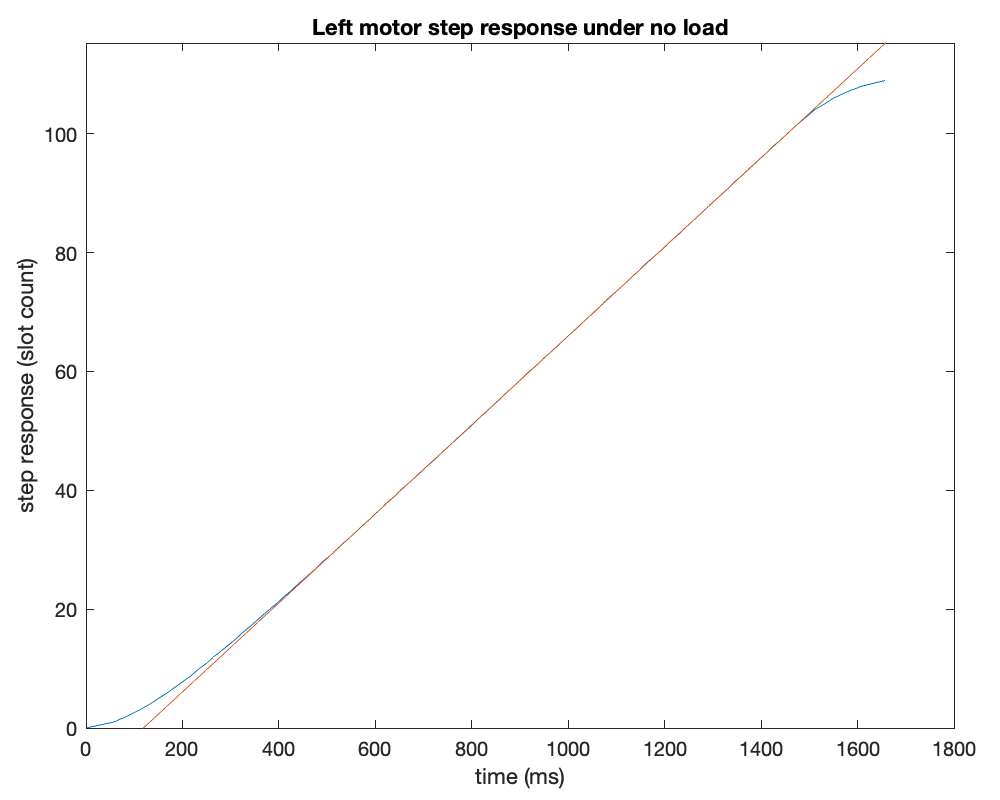
\includegraphics[width=0.5\textwidth]{Identif_left.png} 
		\label{fig:identif_left}
		}
	\quad 
	\subfigure[Silnik prawy bez obciążenia]{
		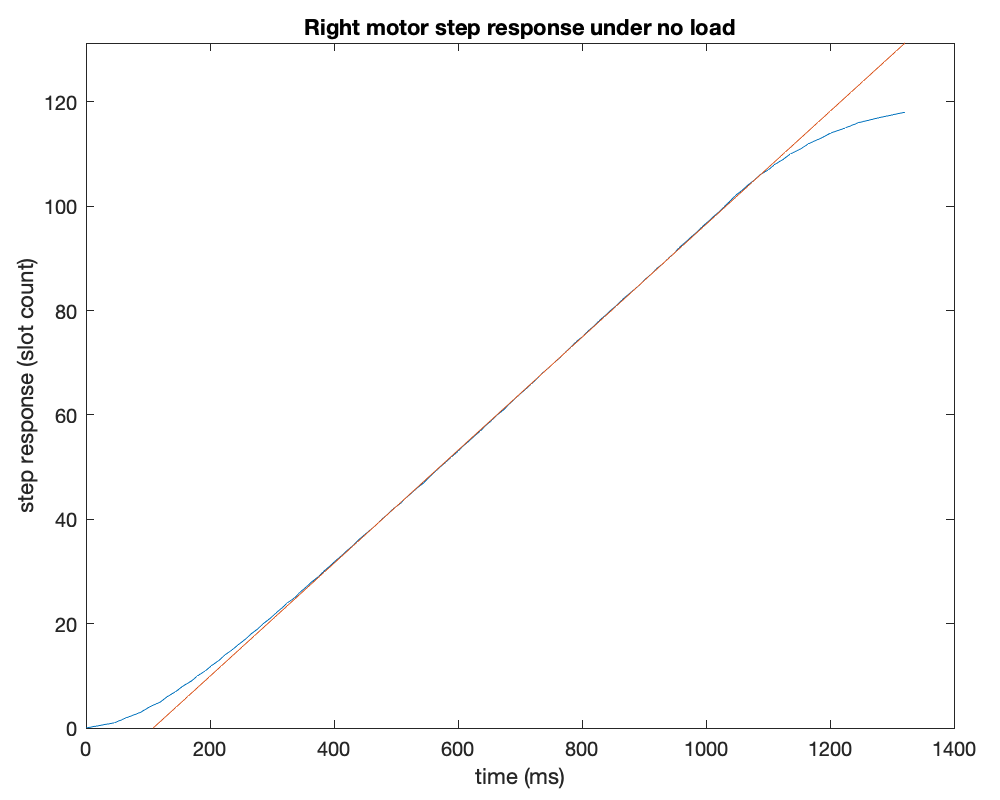
\includegraphics[width=0.5\textwidth]{Identif_right.png}
		\label{fig:identif_rigth} 
	}
	\caption{Wykresy odpowiedzi silników na skok jednostkowy bez obciążenia} 
\end{figure}

\begin{figure}[!htbp] 
	\subfigure[Silnik lewy z obciążeniem podwozia]{
		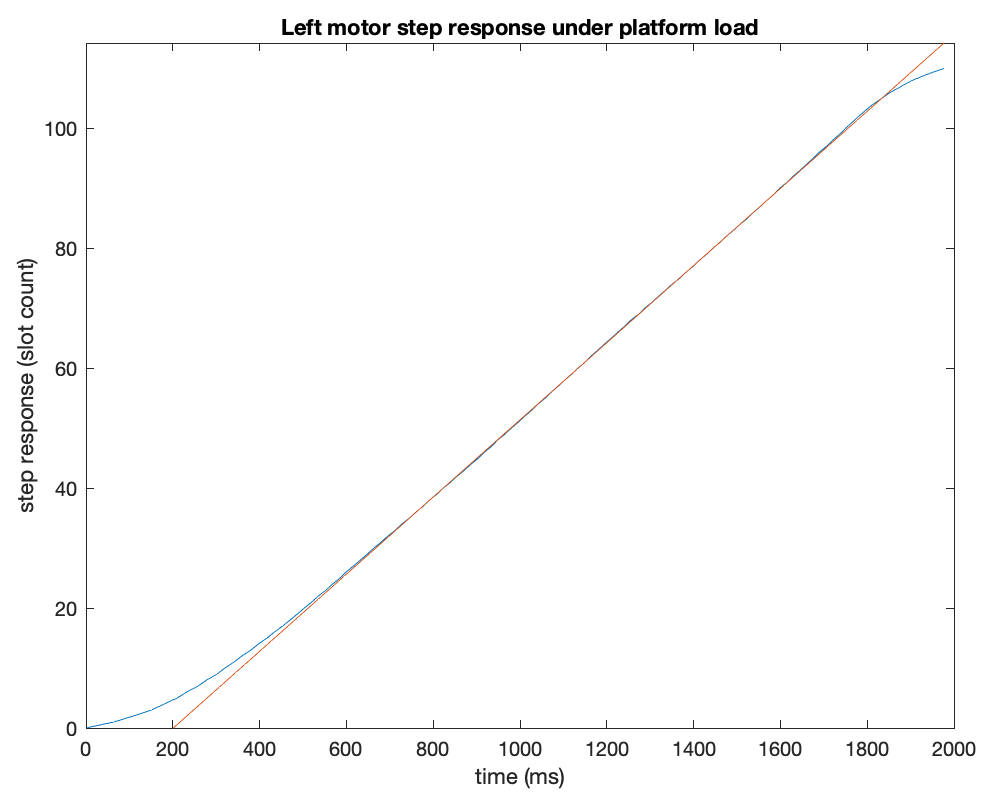
\includegraphics[width=0.5\textwidth]{Identif_left_load.png} 
		\label{fig:identif_left_load}
		}
	\quad 
	\subfigure[Silnik prawy z obciążeniem podwozia]{
		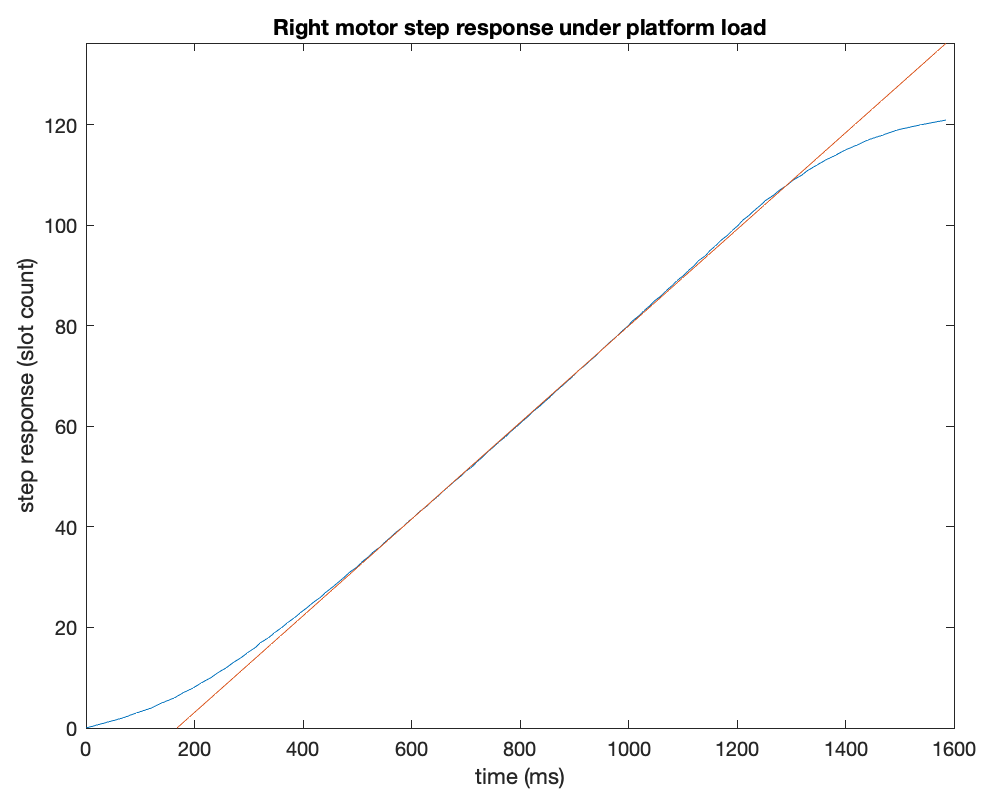
\includegraphics[width=0.5\textwidth]{Identif_right_load.png}
		\label{fig:identif_rigth_load} 
	} 
	\caption{Wykresy odpowiedzi silników na~skok jednostkowy pod obciążeniem podwozia} 
\end{figure}

Ponieważ jako odpowiedź układu zliczano sloty, które są~ekwiwalentem drogi należało spodziewać się odpowiedzi o~charakterze całkującym.
Wyniki identyfikacji potwierdziły te przypuszczenia, wykresy przypominają odpowiedź układu o~transmitancji całki z~inercją.
Można zauważyć, że~odpowiedzi silnika lewego i~prawego różnią się, co~potwierdza obserwacje dotyczącą ich niesymetrycznej pracy.
Widać także, że przy obciążeniu silników podwoziem mają one większą bezwładność, czego również należało się spodziewać.
Podczas strojenia układów regulacji należy bazować na~parametrach obiektów identyfikowanych pod obciążeniem podwozia.
Zaprojektowane układy mają na~celu regulację prędkości, stąd odpowiedź należałoby zróżniczkować aby uzyskać odpowiedź prędkości w~czasie.
Nie jest to~jednak konieczne, zróżniczkowanie odpowiedzi da wykres inercji pierwszego rzędu, z~którego należy odczytać stałą czasową i~wzmocnienie układu.
Te~same parametry da~się określić również z~wykresu odpowiedzi drogi w~czasie.
W~celu ich określenia należy wykreślić prostą do wykresu odpowiedzi.
Punkt przecięcia prostej z~osią \textsc{x} będzie określał stałą czasową układu, natomiast nachylenie prostej jego wzmocnienie.
Ponieważ układ przybliżamy transmitancją całki z~inercją, jego transmitancja będzie miała postać przedstawioną na wzorze \ref{eq:ob_int}.
Parametry stałej czasowej $ T $ i wzmocnienia $ k $, można obliczyć z~dopasowanej do~odpowiedzi prostej, według wzorów \ref{eq:line_param}.

\begin{equation} \label{eq:line_param}
\begin{aligned}
	y(t) &= a \cdot t + b \\
	k &= a \\
	T &= - \frac{a}{b} \\
\end{aligned}
\end{equation}
\begin{equation} \label{eq:ob_int}
	K_{o1} \left( s \right) = \frac{k}{s \left( 1 + sT \right)}
\end{equation}

Identyfikacja układu i~wykresy zostały wykonane w~środowisku \textsc{matlab}, kod programu identyfikacyjnego przedstawia listing \ref{lst:mot_identif}.

\subsection{Strojenie regulatorów}
Ponieważ regulatory \textsc{PI} będą regulowały prędkość silników należy przekształcić odpowiedź tak by~uzyskać wykres prędkości w~czasie.
Uzyskana identyfikacja obiektu całkującego opisuje zmiany drogi w~czasie, aby uzyskać transmitancję związaną ze~zmianami prędkości należy zróżniczkować transmitancję obiektu całkującego przemnażając ją~przez operator $ s $, co~obrazują przekształcenia we~wzorze \ref{eq:ob_inert}. Jak widać zmiany prędkości w~czasie są~opisane modelem inercyjnym.

\begin{equation} \label{eq:ob_inert}
	K_{o2} \left( s \right) = s \cdot K_{o1} \left( s \right) = s \cdot \frac{k}{s \left( 1 + sT \right)} = \frac{k}{1 + sT}
\end{equation}

Zdecydowano się na~regulator \textsc{PI}, który ma~wystarczający astatyzm, oraz jest łatwy w~implementacji.
W przypadku naszego układu, który opisujemy transmitancją niskiego rzędu odpowiednim sposobem strojenia będzie użycie lini pierwiastkowych.
W celu wykreślenia linii najlepiej zapisać transmitancję regulatora i~obiektu w postaci zero-biegunowej, którą przedstawia wzór \ref{eq:reg_pi_casc}.

\begin{equation} \label{eq:reg_pi_casc}
	PI \left( s \right) \cdot K_{o2} \left( s \right) = \left( \frac{s + c}{s} \right) \cdot \frac{k}{1 + sT}
\end{equation}

Należy zdecydować o~wartości dodanego zera $ c $. Jego stosunek do~stałej czasowej $ T $ zdecyduje o~kształcie linii pierwiastkowych.
Można rozpatrzeć trzy przypadki:
\begin{itemize}
	\item zero większe do~stałej czasowej: $ c > T $,
	\item zero równe stałej czasowej: $ c = T $
	\item zero mniejsze od~stałej czasowej: $ c < T $.
\end{itemize}
Przypadek równości tych parametrów jest najbardziej korzystny, doprowadzi do~skrócenia fragmentów transmitancji, w~takim wypadku regulator działałby jak korektor, a~układ byłby najszybszym z~możliwych.
Mimo tego jest to~przypadek, który należy odrzucić.
Aby osiągnąć równość parametrów należałoby przeprowadzić identyfikację o~nieosiągalnej dokładności, jednak wyznaczona wartość stałej czasowej może, i~zapewne różni się od~rzeczywistych parametrów układu.
Mało prawdopodobne jest zrealizowanie korektora, a~dobór zera równego zidentyfikowanej stałej czasowej da w~rzeczywistości niespodziewane rezultaty, ze~względu na~niedoskonałości procesu identyfikacji.
Należy rozpatrzyć pozostałe dwa przypadki, liniowe pierwiastkowe dla nich wykreślono na rysunkach \ref{fig:root_loc_fast} oraz \ref{fig:root_loc_slow}. Program kreślącey linie pierwiastkowe w~środowisku \textsc{matlab}, na~podstawie identyfikacji obiektu przedstawia listing \ref{lst:root_loc}.

\begin{figure}[!htbp] 
	\subfigure[Wariant z zerem większym od stałej czasowej]{% 
		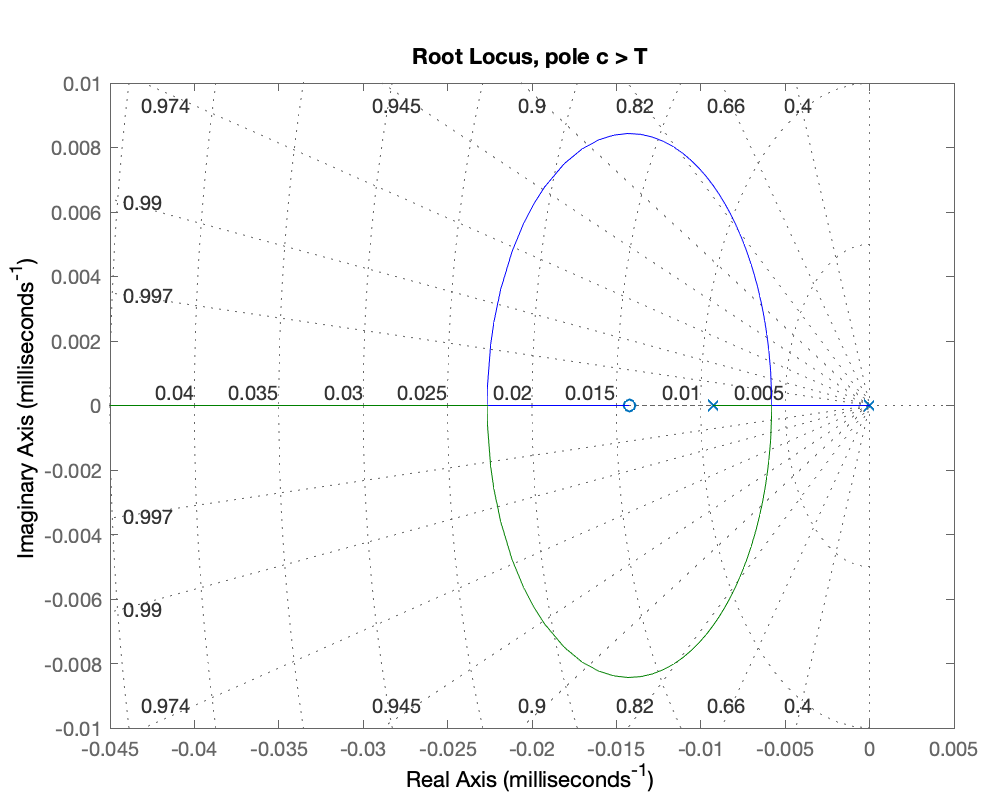
\includegraphics[width=0.5\textwidth]{Root_loc_fast.png} 
		\label{fig:root_loc_fast}
		}
	\quad 
	\subfigure[Wariant z zerem mniejszym od stałej czasowej]{% 
		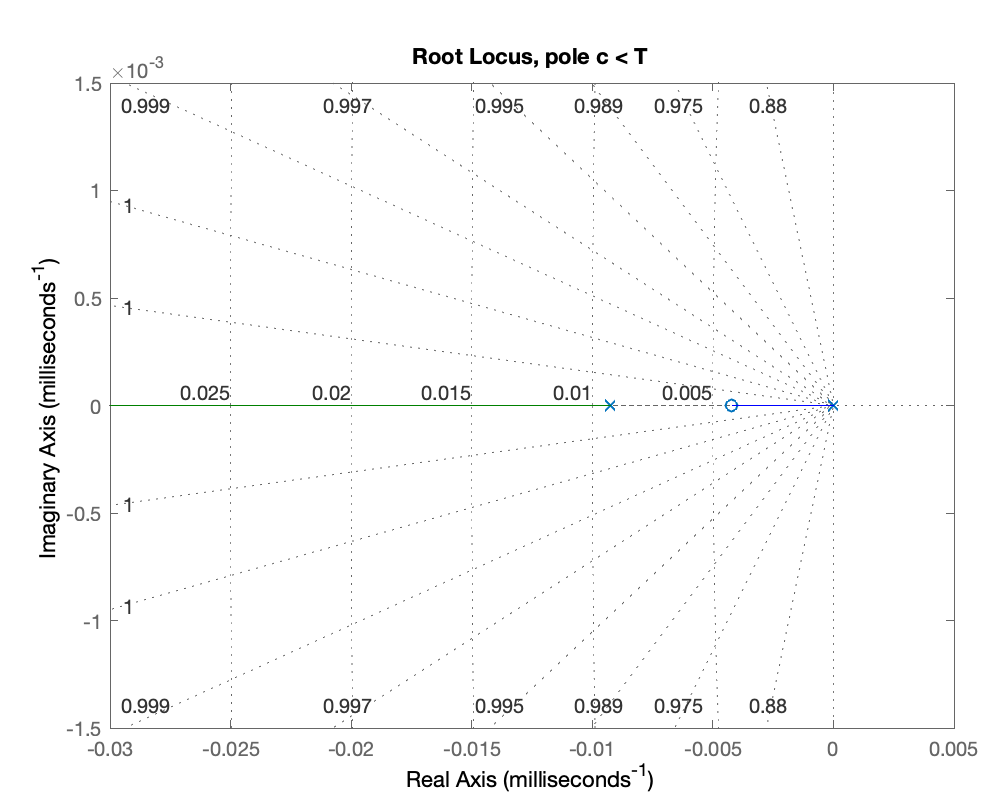
\includegraphics[width=0.5\textwidth]{Root_loc_slow.png}
		\label{fig:root_loc_slow} 
	} 
	\caption{Rozpatrywane linie pierwiastkowe układu z regulatorem \textsc{pi}} 
\end{figure}

\begin{listing}[htb]
\caption{Program kreślący linie pierwiastkowe układu na podstawie identyfikacji obiektu}
\inputminted[firstline=1, lastline=32, frame=lines, linenos, breaklines]{matlab}{../Identification/Identification.m}
\label{lst:root_loc}
\end{listing}

Prędkość działania finalnego układu jest zdeterminowana przez położenie bieguna, który znajduje się najbliżej osi urojonej~\textsc{y}.~Im~bardziej od~osi oddalony jest ten biegun tym szybszy układ.
Przy analizie linii pierwiastkowych należy również pamiętać, że~położenia biegunów o~niezerowej części urojonej oznaczają oscylacje układu.
Jak wspomniano w~sekcji~\ref{sec:err} zależy nam na~konstrukcji układu aperiodycznego\footnote{tzn. bez oscylacji.}, czyli powinniśmy umieścić nasze bieguny na~osi~\textsc{x}.

Można zauważyć że~przypadek $ c > T $~pozwala na~zbudowanie szybszego regulatora.
W takiej konfiguracji, przy dużych wzmocnieniach najwolniejszy biegun znajduje się z~lewej strony założonego zera, czyli dalej od~osi urojonej \textsc{y}.
W~konfiguracji $ c < T $~najwolniejszy biegun znajduje się po~prawej stronie zera, czyli taki układ jest wolniejszy.
Przypadek $ c > T $~zdaje się bardziej korzystny, jednak niesie ze~sobą ryzyko oscylacji.
Teoretycznie najlepsze położenie bieguna w~tej konfiguracji to~miejsce w~którym pierwiastki wracają z~koła wartości urojonych z~powrotem na~oś~rzeczywistą \textsc{x}.
Jest to~jednak lokacja ryzykowna ze~względu na niedoskonałości identyfikacji.
Przez jej błędy możemy omyłkowo, w~układzie rzeczywistym, ulokować bieguny z~częścią urojoną, czyli wprowadzić oscylacje.
Dla pewności wyeliminowania oscylacji należy zwiększyć wzmocnienie układu i~umieścić pierwiastki dalej od~koła wartości urojonych.
Wadą takiego rozwiązania jest spowolnienie układu przez zbliżenie bieguna do~osi~\textsc{y}~oraz wymaganie dużego wzmocnienia, które może być niemożliwe dla układu realizującego algorytm sterowania i~elementów wykonawczych.
Konfiguracja $ c < T $ może być praktycznie lepsza, niż mogło zdawać się pierwotnie, nie niesie ryzyka oscylacji.
Fakt, że taka konfiguracja jest wolniejsza niesie pewne zalety, mało gwałtowne ruchy robota minimalizują ryzyko poślizgów kół.
W~celu nastrojenia układów regulacji należy wykonać eksperymenty i~porównać oczekiwania wynikające z~linii pierwiastkowych z~rzeczywistością.

\section{Implementacja programistyczna}
\subsection{Podział i organizacja kodu}
Kod odpowiadający za~różne funkcjonalności robota umieszczono w~oddzielnych plikach, w~których znajdują się funkcje budujące warstwy abstrakcji peryferiów konstrukcji. Zdecydowano się na~następujący podział plików i~funkcji:
\begin{itemize}
	\item \texttt{defines} zawiera stałe programu oraz makroinstrukcje,
	\item \texttt{servoSensor} zawiera funkcje budujące warstwę abstrakcji czujnika ultradźwiękowego na wieży serwomechanizmu, pozwala na~kierowanie czujnika w~różne strony, wykrywanie przeszkód oraz poszukiwanie wolnej drogi w~otoczeniu,
	\item \texttt{platformMotors} zawiera funkcje budujące warstwę abstrakcji platformy robota, pozwala na~jazdę na~wprost oraz skręty, bazuje w~działaniu na układach regulacji,
	\item \verb|HC_SR04| zawiera zmodyfikowaną bibliotekę obsługi czujnika ultradźwiękowego w~trybie nieblokującym, biblioteka jest wykorzystywana przez funkcje z~pliku \texttt{servoSensor},
	\item \texttt{main} zawiera główną logikę programu, wywołuje funkcje poszukiwań drogi bez przeszkód i~podążania w~tym kierunku, kontroluje także wyłączanie i~włączanie układu po~odebraniu rozkazów wysłanych podczerwienią.
\end{itemize}

\subsection{Algorytm omijania przeszkód}
Kluczowym elementem omijania przeszkód jest znajdywanie drogi, na~której nie znajdują się przeszkody.
Proces znajdywania nowego kierunku jazdy rozpoczyna się w~momencie, w~którym na obecnym kierunku jazdy zostaje wykryta przeszkoda.
Wtedy robot się zatrzymuje i~losuje po której stronie najpierw będzie szukał wolnej drogi. Potem zwraca w~tym kierunku czujnik ultradźwiękowy i~wykrywa obecność przeszkód.
Jeżeli te~nie zostaną wykryte platforma skręca w~wylosowanym kierunku i~rozpoczyna jazdę na wprost.
W przeciwnym przypadku robot kieruje czujnik w~przeciwną stronę i~bada czy tam znajduje się przeszkoda, jeżeli nie to~rozpocznie jazdę w~tym kierunku.
Kiedy obie strony robota są~zablokowane ten zwróci się w~kierunku z~którego przyjechał. Opisane zachowanie obrazuje schemat na~rysunku~\ref{fig:tikz:pathfind_flowchart}.
\begin{figure}[htbp]
	\centering
	\scalebox{0.8}{\documentclass{standalone}

\usepackage{tikz}
\usetikzlibrary{shapes, arrows}
\usetikzlibrary{arrows.meta, positioning}
\begin{document}

% Define styles
\tikzstyle{startstop} = [rectangle, rounded corners, minimum width=3cm, minimum height=1cm,text centered, draw=black]
\tikzstyle{process} = [rectangle, minimum width=3cm, minimum height=1.25cm, text centered, draw=black]
\tikzstyle{decision} = [diamond, aspect=3, minimum width=3cm, minimum height=1cm, text centered, draw=black]

\begin{tikzpicture}[auto, node distance=2cm, >=latex']
	\node (start) [startstop] {Start};
	\node (rand) [process, below of=start] {
	\small{\texttt{int direction = random(RIGHT, LEFT + 1);}}
	};
	\node (turn) [process, below of=rand] {
	\small{\texttt{turnServoSensor(direction);}}
	};
	\node (pathfind) [decision, below of=turn, yshift=-1cm] {
	\small{\texttt{sensor.probeRange()<SAFE\_DIST;}}
	};
	\node (return) [process, right of=pathfind, yshift=-2.5cm, xshift=2.5cm] {
	\begin{tabular}{c}
		\small{\texttt{direction = !direction;}} \\ 
		\small{\texttt{turnServoSensor(direction);}}
	\end{tabular}
	};
	\node (repathfind) [decision, below of=return, yshift=-1cm] {
	\small{\texttt{sensor.probeRange()<SAFE\_DIST;}}
	};
	\node (back) [process, right of=repathfind, yshift=-2.5cm, xshift=2.5cm] {
	\small{\texttt{direction = BACK;}}
	};
	\node (finish) [process, left of=back, xshift=-11.5cm] {
	\begin{tabular}{c}
		\small{\texttt{turnServoSensor(FRONT);}} \\ 
		\small{\texttt{return direction;}}
	\end{tabular}
	};
	\node (stop) [startstop, below of=finish] {Stop};
	
	\draw [->] (start) -- node {} (rand);
	\draw [->] (rand) -- node {} (turn);
	\draw [->] (turn) -- node {} (pathfind);
	\draw [->] (pathfind.west) -| node[yshift=0.25cm, xshift=0.25cm] {No} (finish);
	\draw [->] (pathfind) -| node[yshift=0.25cm, xshift=-1cm] {Yes} (return);
	\draw [->] (return) -- node {} (repathfind);
	\draw [->] (repathfind) -| node[yshift=0.25cm, xshift=-1cm] {Yes} (back);
	\draw [->] (repathfind) -| node[yshift=0.25cm, xshift=4cm] {No} (finish);
	\draw [->] (back) -- node {} (finish);
	\draw [->] (finish) -- node {} (stop);
	
\end{tikzpicture}

\end{document}}
	\caption{Schemat blokowy algorytmu znajdywania kierunku bez przeszkód}
	\label{fig:tikz:pathfind_flowchart}
\end{figure}

\subsection{Algorytmy regulacji}
\subsubsection{Algorytm regulacji synchronizacji prędkości silników}
Algorytm synchronizacji został zaprogramowany według schematu na~rysunku \ref{fig:tikz:pathfind_flowchart}.
Kod realizujący założenia schematu przedstawiono na~listingu \ref{lst:synch_reg}.
Parametry regulatora należy przekształcić względem tych uzyskanych z~analizy linii pierwiastkowych, aby ułatwić obliczenia i~czytelność kodu.
Formuła regulatora zastosowana w~kodzie ma postać jak we~wzorze \ref{eq:progr_PI}, gdzie:
\begin{itemize}
	\item $ \Delta \alpha $ to~uchyb ilości zliczonych slotów,
	\item $ \Delta \omega $ to~uchyb chwilowej prędkości,
\end{itemize}
Parametry regulatora w takiej postaci można wyliczyć według wzoru \ref{eq:reg_param}, gdzie:
\begin{itemize}
	\item $ k_r $ to wzmocnienie regulatora odczytane z~linii pierwiastkowych,
	\item $ c $ to~wartość zera transmitacnji ze~wzoru \ref{eq:reg_pi_casc}.
\end{itemize}

\begin{equation} \label{eq:reg_param}
\begin{aligned}
	P &=  k_r\\
	I &=  k_r \cdot c\\
\end{aligned}
\end{equation}

\begin{equation} \label{eq:progr_PI}
	PI \left( \Delta \alpha, \Delta \omega \right) = P \cdot \Delta \alpha + I \cdot \Delta \omega
\end{equation}

\begin{listing}[htb]
\caption{Algorytm regulacji synchronizacji prędkości silników}
\inputminted[firstline=161, lastline=183, frame=lines, linenos, breaklines]{cpp}{../src/platformMotors.cpp}
\label{lst:synch_reg}
\end{listing}

\subsubsection{Algorytm regulacji skrętu o~kąt zadany}
Algorytm regulacji skrętu o~kąt zadany został zaprogramowany według schematu na~rysunku~\ref{fig:tikz:control_block_casc}.
Kod pętli wewnątrz której realizowana jest regulacja przedstawiony jest na~listingu~\ref{lst:rot_reg}.
Wypracowanie sterowania rozpoczyna się od~wyznaczenia uchybu ilości slotów wymaganych do~wykonania obrotów.
Wartość zadana \texttt{target} regulatora położenia jest wyliczana z~makrofunkcji realizującej wzór~\ref{eq:slot_num}.
Wartość zadana prędkości została ograniczona, aby zapobiec poślizgom.
Wartość zadana regulatora prędkości jest wypracowywana przez regulator położenia.
Różniczkowanie ilości slotów w~celu otrzymania prędkości chwilowej zrealizowano przez odwracanie czasu zliczonego między ostatnimi przerwaniami wygenerowanymi przez czujniki szczelinowe.
Kod przerwań czujników przedstawia listing \ref{lst:enc_int}
Istotne jest aby pamiętać o~rzutowaniu wartości \texttt{int} na~\texttt{float} przy dzieleniu, aby zachować precyzję obliczeń.
Całkowanie uchybu odbywa się przez mnożenie go~przez czas jaki upłynął od~ostatniego przerwania czujnika szczelinowego.
W~rozdziale \ref{sec:reg_casc} opisującym założenia budowy regulatora kaskadowego przedstawiono pomysł konstrukcji zerującej wartość całki przy każdym przerwaniu czujnika szczelinowego.
Odpowiednikiem tego założenia w~kodzie jest brak zapamiętywania i~sumowania poprzednich wartości całki, przy każdej nowej szczelinie czas od~tego przerwania jest liczony od~nowa.
Jest to bardzo uproszczona realizacja członu całkującego, jednak zupełnie wystarczająca w~naszym przypadku\footnote{
	Działanie członu całkującego można sprawdzić w sposób eksperymentalny.
	W tym celu wyłączono człon proporcjonalny, zerując jego parametr \texttt{P}.
	Robot powinien na początku nie ruszyć, a~wraz z~brakiem jego ruchu powinien być całkowany coraz większy uchyb i~zadawane coraz większe wysterowanie silników.
	Po~chwili powinien być słyszany odgłos silników próbujących pokonać opory ruchu.
	Ostatecznie wartość całki powinna być na tyle duża, że~silniki ruszą i~nastąpi obrót kół o~kąt powodujący zliczenie jednej szczeliny.
	Ponieważ całkę zerujemy przy każdej zliczonej szczelinie, robot się zatrzyma i~zacznie całkować uchyb od~nowa.
	Proces ten będzie powtarzał się aż~robot wykona stopniowo pełen skręt.
	Przewidywania te~potwierdził eksperyment.
}.

\begin{listing}[htb]
\caption{Algorytm regulacji skrętu o kąt zadany}
\inputminted[firstline=85, lastline=126, frame=lines, linenos, breaklines, fontsize=\small ]{cpp}{../src/platformMotors.cpp}
\label{lst:rot_reg}
\end{listing}

\subsection{Kod funkcji obsługującej przerwanie czujnika szczelinowego}
Kod funkcji obsługującej przerwanie czujnika szczelinowego\footnote{Funkcje obsługi przerwań lewego i~prawego czujnika należało napisać oddzielnie, ale ich kod jest praktycznie taki sam.
Opisano tu kod obsługi jednego czujnika, ale drugi różni się tylko operacjami na innych zmiennych globalnych, logika jego działania jest identyczna.} przedstawiono na listingu \ref{lst:enc_int}.
Funkcje obsługi przerwań czujników szczelinowych mają za~zadanie inkrementację licznika szczelin oraz obliczenie czasu od ostatniego przerwania.
W funkcji należało uwzględnić inne zachowanie przerwań przy początku ruchu robota.
Przy testach czujników okazało się, że~przy zmianie stanu czujnika następuje zjawisko podobne do~odbijania styków, co~sprawiało że~fałszywie zliczana była duża ilość szczelin.
Aby temu zapobiec ignorowane są sygnały które pojawiły się zbyt szybko względem ostatniej zmiany.
Tworząc kod przerwań należy pamiętać, że~ich obsługa w~mikrokontrolerach ATmega wyłącza działanie liczników, przez co~funkcje \texttt{millis()} w~przerwaniach zwracają czas włączenia przerwania, a~czas który upłynął na obsłudze przerwania jest pomijany przy następnych wywołaniach funkcji \texttt{millis()}.
To zjawisko mogłoby powodować błędy jeżeli zależałoby nam na~precyzyjnym zliczaniu czasu od~wydarzenia, kiedy podczas zliczania obsługujemy dużo przerwań o~długim kodzie obsługi.
Taka potrzeba nie zachodzi jednak w~naszym przypadku, więc użycie funkcji \texttt{millis()} w~kodzie obsługi przerwań jest bezpieczne.

\begin{listing}[htb]
\caption{Kod funkcji obsługującej przerwanie czujnika szczelinowego}
\inputminted[firstline=185, lastline=206, frame=lines, linenos, breaklines]{cpp}{../src/platformMotors.cpp}
\label{lst:enc_int}
\end{listing}

\section{Wykorzystane technologie}
\subsection{Narzędzia programistyczne}
Ze względu na~ograniczenia programu Arduino IDE~zdecydowano się na~użycie środowiska PlatformIO\footnote{PlatformIO: \url{https://platformio.org}}, które jest wtyczką do programu Visual Studio Code\footnote{Visual Studio Code: \url{https://code.visualstudio.com}}. Taka konfiguracja oferuje:
\begin{itemize}
	\item bogate kolorowanie składni języków programowania,
	\item zaawansowany system autouzupełniania kodu z~użyciem technologii \textit{IntelliSense},
	\item automatyczne wykrywanie portów szeregowych z~podłączonymi płytkami,
	\item konstrukcja bazująca na plikach \textit{make} i~programie \textsc{avrdude}.
\end{itemize}
Kod projektu wersjonowano z~użyciem programu Git oraz korzystając z~usług serwisu GitHub, który oferuje internetowy interfejs do~zarządzania repozytorium, system \textit{issue tracking} oraz zarządzanie projektem za~pomocą tablic kanban.

\subsection{Komunikacja z mikroprocesorem}
Do komunikacji z~mikroprocesorem przydatny okazał się program \textsc{avrdude}.
Szczególnie jego polecenia testu poprawnej komunikacji i~odczytu \textit{fuse bitów}.
Poniżej przedstawiono przykład użycia polecenia testu mikrokontrolera oraz jego wynik:

\begin{verbatim}
$ sudo avrdude -p m32u4 -c usbasp -P usb
avrdude: AVR device initialized and ready to accept instructions
Reading | ############################################### | 100% 0.01s
avrdude: Device signature = 0x1e9587
avrdude: safemode: Fuses OK
avrdude done.  Thank you.
\end{verbatim}
Polecenie odczytu \textit{fusebitów} ma z kolei następujący format i~daje wynik:
\begin{verbatim}
$ sudo avrdude -p m32u4 -c usbasp -P usb -U hfuse:r:hfuse.hex:h
avrdude: AVR device initialized and ready to accept instructions
Reading | ############################################### | 100% 0.01s
avrdude: Device signature = 0x1e9587
avrdude: reading hfuse memory:
Reading | ############################################### | 100% 0.00s
avrdude: writing output file "hfuse.hex"
avrdude: safemode: Fuses OK
avrdude done.  Thank you.
\end{verbatim}
Jak widać w powyższych instrukcjach, do programowania mikrokontrolera użyto programatora USBasp.
Przy zakupie takiego programatora warto upewnić się, że~kupujemy wersję z~najnowszym firmwarem, dzięki czemu programator będzie miał od razu dostępną funkcję automatycznego dopasowania do taktowania zegara mikrokontrolera.
Program Arduino IDE pozwala na wypalenie w~pamięci mikrokontrolera bootloadera Arduino.
Opcja ta~jest dostępna w~pasku menu w~zakładce narzędzia.

\section{Perspektywy rozwoju, podsumowanie}
Wykonany projekt spełnił założenia, dzięki zastosowaniu układów regulacji napędu silników robot jest stanie poruszać się na~tyle precyzyjnie by~wymijać przeszkody.
Wszystkie elementy układu oraz części obwodu drukowanego działają w~sposób poprawny.
Załączniki do dokumentacji zawierają materiały multimedialne prezentujące osiągniętą dokładność pracy robota.
Projekt miał charakter edukacyjny, jego wyników nie da się porównać z~produktami komercyjnymi, jednak zdobyte podczas jego realizacji doświadczenie i~fragmenty pracy mogą być przydatne przy konstrukcji robotów magazynowych, robotów labiryntowych oraz przy budowie dedykowanych serwomechanizmów.

Precyzję układu można zwiększyć stosując tarcze enkoderów o~większej ilości szczelin, lub stosując enkodery umieszczane przed przekładnią silników.
Ciekawą ścieżką rozwoju może być zamiana układu pomiarowego z~enkodera badającego obroty kół na system \textit{Yaw, Pitch Roll}.
Jest to~zestaw współpracujących ze sobą: żyroskopu, akcelerometru oraz magnetometru w~celu ustalenia kierunku układu w~przestrzeni poprzez kąty Eulera.
Taki układ pomiarowy cechowałby się daleko większą dokładnością i~obejmowałby pętlą sprzężenia zwrotnego nie tylko obroty silnika, ale rzeczywisty kierunek robota, eliminując błędy związane z~poślizgiem kół.
Na obecnym etapie projektu taki system pomiarowy znacząco przekroczyłby budżet, jednak w~przyszłości może on~stanowić ciekawe zagadnienie.
Jego wprowadzenie pozwoliłoby na~zachowanie sporej ilości aktualnego kodu, zmiany wymagałby jedynie tor pomiarowy i~zadajnik.

Na bieżącym etapie układ nie zapamiętuje ścieżki którą przebył, aby to~zmienić można skonstruować drzewo binarne wykonanych skrętów i~odległości między nimi.
Dzięki temu układ mógłby analizować przebytą drogę i~szukać wyjścia z~bardziej złożonych labiryntów.
Kod programu, pliki Autodesk Eagle oraz dokumentacja są dostępne na stronie GitHub projektu: \url{https://github.com/MaciejZj/MazeBot}.

\begin{thebibliography}{9}

\bibitem{baranowski}
Rafał Baranowski,
\textit{Mikrokontrolery AVR ATmega w praktyce}
Wydawnictwo BTC, Warszawa 2005

\bibitem{wegrzyn}
Stefan Węgrzyn,
\textit{Podstawy automatyki}
Państwowe Wydawnictwo Naukowe, Warszawa 1974.

\bibitem{takashi}
Y. Takashi, M.J. Rabins, D.M. Auslander,
\textit{STEROWANIE i systemy dynamiczne},
Wydawnictwo Naukowo Techniczne, Warszawa 1976.

\bibitem{Buch_measure}
Praca zbiorowa pod redakcją Dariusza Buchczika i Stanisława Walusia,
\textit{Laboratorium Podstaw Miernictwa},
Wydawnictwo Politechniki Śląskiej, Gliwice 2014.

\bibitem{resnick_phys}
David Halliday, Robert Resnick, Jearl Walker,
\textit{Podstawy Fizyki. Tom 1},
Wydawnictwo Naukowe PWN, Warszawa 2003.

\bibitem{atmega32u4_datasheet}
Atmel: \textit{ATmega16U4/ATmega32U4 8-bit Microcontroller with 16/32K bytes of ISP Flash and USB Controller}, \url{http://ww1.microchip.com/downloads/en/devicedoc/atmel-7766-8-bit-avr-atmega16u4-32u4\_datasheet.pdf}

\bibitem{h_bridge_datasheet}
STMicroelectronics: \textit{L298
DUAL FULL-BRIDGE DRIVER}, \url{https://www.sparkfun.com/datasheets/Robotics/L298_H_Bridge.pdf}

\bibitem{ultr_datasheet}
Elec: \textit{Ultrasonic Ranging Module HC - SR04}, \url{https://www.mouser.com/ds/2/813/HCSR04-1022824.pdf}

\bibitem{ir_datasheet}
Vishay: \textit{TSOP48 Photo Modules for PCM Remote Control Systems}, \url{http://mkpochtoi.narod.ru/TSOP4836_ds.pdf}

\bibitem{stab_datasheet}
STMicroelectronics: \textit{TL7800 series positive voltage regulators}, \url{https://datasheet.octopart.com/L7805CV-STMicroelectronics-datasheet-7264666.pdf}

\bibitem{ziolo}
Praca zbiorowa pod redakcją Krzysztofa Zioło
\textit{LABORATORIUM ELEKTRONIKI I Elementy półprzewodnikowe i układy podstawowe}.
Wydanie III zmienione .
Wydawnictwo Politechniki Śląskiej, Gliwice 1999.

\end{thebibliography}
\end{document}